% Options for packages loaded elsewhere
\PassOptionsToPackage{unicode}{hyperref}
\PassOptionsToPackage{hyphens}{url}
\PassOptionsToPackage{dvipsnames,svgnames,x11names}{xcolor}
%
\documentclass[
  letterpaper,
  DIV=11,
  numbers=noendperiod]{scrreprt}

\usepackage{amsmath,amssymb}
\usepackage{iftex}
\ifPDFTeX
  \usepackage[T1]{fontenc}
  \usepackage[utf8]{inputenc}
  \usepackage{textcomp} % provide euro and other symbols
\else % if luatex or xetex
  \usepackage{unicode-math}
  \defaultfontfeatures{Scale=MatchLowercase}
  \defaultfontfeatures[\rmfamily]{Ligatures=TeX,Scale=1}
\fi
\usepackage{lmodern}
\ifPDFTeX\else  
    % xetex/luatex font selection
\fi
% Use upquote if available, for straight quotes in verbatim environments
\IfFileExists{upquote.sty}{\usepackage{upquote}}{}
\IfFileExists{microtype.sty}{% use microtype if available
  \usepackage[]{microtype}
  \UseMicrotypeSet[protrusion]{basicmath} % disable protrusion for tt fonts
}{}
\makeatletter
\@ifundefined{KOMAClassName}{% if non-KOMA class
  \IfFileExists{parskip.sty}{%
    \usepackage{parskip}
  }{% else
    \setlength{\parindent}{0pt}
    \setlength{\parskip}{6pt plus 2pt minus 1pt}}
}{% if KOMA class
  \KOMAoptions{parskip=half}}
\makeatother
\usepackage{xcolor}
\setlength{\emergencystretch}{3em} % prevent overfull lines
\setcounter{secnumdepth}{5}
% Make \paragraph and \subparagraph free-standing
\makeatletter
\ifx\paragraph\undefined\else
  \let\oldparagraph\paragraph
  \renewcommand{\paragraph}{
    \@ifstar
      \xxxParagraphStar
      \xxxParagraphNoStar
  }
  \newcommand{\xxxParagraphStar}[1]{\oldparagraph*{#1}\mbox{}}
  \newcommand{\xxxParagraphNoStar}[1]{\oldparagraph{#1}\mbox{}}
\fi
\ifx\subparagraph\undefined\else
  \let\oldsubparagraph\subparagraph
  \renewcommand{\subparagraph}{
    \@ifstar
      \xxxSubParagraphStar
      \xxxSubParagraphNoStar
  }
  \newcommand{\xxxSubParagraphStar}[1]{\oldsubparagraph*{#1}\mbox{}}
  \newcommand{\xxxSubParagraphNoStar}[1]{\oldsubparagraph{#1}\mbox{}}
\fi
\makeatother

\usepackage{color}
\usepackage{fancyvrb}
\newcommand{\VerbBar}{|}
\newcommand{\VERB}{\Verb[commandchars=\\\{\}]}
\DefineVerbatimEnvironment{Highlighting}{Verbatim}{commandchars=\\\{\}}
% Add ',fontsize=\small' for more characters per line
\usepackage{framed}
\definecolor{shadecolor}{RGB}{241,243,245}
\newenvironment{Shaded}{\begin{snugshade}}{\end{snugshade}}
\newcommand{\AlertTok}[1]{\textcolor[rgb]{0.68,0.00,0.00}{#1}}
\newcommand{\AnnotationTok}[1]{\textcolor[rgb]{0.37,0.37,0.37}{#1}}
\newcommand{\AttributeTok}[1]{\textcolor[rgb]{0.40,0.45,0.13}{#1}}
\newcommand{\BaseNTok}[1]{\textcolor[rgb]{0.68,0.00,0.00}{#1}}
\newcommand{\BuiltInTok}[1]{\textcolor[rgb]{0.00,0.23,0.31}{#1}}
\newcommand{\CharTok}[1]{\textcolor[rgb]{0.13,0.47,0.30}{#1}}
\newcommand{\CommentTok}[1]{\textcolor[rgb]{0.37,0.37,0.37}{#1}}
\newcommand{\CommentVarTok}[1]{\textcolor[rgb]{0.37,0.37,0.37}{\textit{#1}}}
\newcommand{\ConstantTok}[1]{\textcolor[rgb]{0.56,0.35,0.01}{#1}}
\newcommand{\ControlFlowTok}[1]{\textcolor[rgb]{0.00,0.23,0.31}{\textbf{#1}}}
\newcommand{\DataTypeTok}[1]{\textcolor[rgb]{0.68,0.00,0.00}{#1}}
\newcommand{\DecValTok}[1]{\textcolor[rgb]{0.68,0.00,0.00}{#1}}
\newcommand{\DocumentationTok}[1]{\textcolor[rgb]{0.37,0.37,0.37}{\textit{#1}}}
\newcommand{\ErrorTok}[1]{\textcolor[rgb]{0.68,0.00,0.00}{#1}}
\newcommand{\ExtensionTok}[1]{\textcolor[rgb]{0.00,0.23,0.31}{#1}}
\newcommand{\FloatTok}[1]{\textcolor[rgb]{0.68,0.00,0.00}{#1}}
\newcommand{\FunctionTok}[1]{\textcolor[rgb]{0.28,0.35,0.67}{#1}}
\newcommand{\ImportTok}[1]{\textcolor[rgb]{0.00,0.46,0.62}{#1}}
\newcommand{\InformationTok}[1]{\textcolor[rgb]{0.37,0.37,0.37}{#1}}
\newcommand{\KeywordTok}[1]{\textcolor[rgb]{0.00,0.23,0.31}{\textbf{#1}}}
\newcommand{\NormalTok}[1]{\textcolor[rgb]{0.00,0.23,0.31}{#1}}
\newcommand{\OperatorTok}[1]{\textcolor[rgb]{0.37,0.37,0.37}{#1}}
\newcommand{\OtherTok}[1]{\textcolor[rgb]{0.00,0.23,0.31}{#1}}
\newcommand{\PreprocessorTok}[1]{\textcolor[rgb]{0.68,0.00,0.00}{#1}}
\newcommand{\RegionMarkerTok}[1]{\textcolor[rgb]{0.00,0.23,0.31}{#1}}
\newcommand{\SpecialCharTok}[1]{\textcolor[rgb]{0.37,0.37,0.37}{#1}}
\newcommand{\SpecialStringTok}[1]{\textcolor[rgb]{0.13,0.47,0.30}{#1}}
\newcommand{\StringTok}[1]{\textcolor[rgb]{0.13,0.47,0.30}{#1}}
\newcommand{\VariableTok}[1]{\textcolor[rgb]{0.07,0.07,0.07}{#1}}
\newcommand{\VerbatimStringTok}[1]{\textcolor[rgb]{0.13,0.47,0.30}{#1}}
\newcommand{\WarningTok}[1]{\textcolor[rgb]{0.37,0.37,0.37}{\textit{#1}}}

\providecommand{\tightlist}{%
  \setlength{\itemsep}{0pt}\setlength{\parskip}{0pt}}\usepackage{longtable,booktabs,array}
\usepackage{calc} % for calculating minipage widths
% Correct order of tables after \paragraph or \subparagraph
\usepackage{etoolbox}
\makeatletter
\patchcmd\longtable{\par}{\if@noskipsec\mbox{}\fi\par}{}{}
\makeatother
% Allow footnotes in longtable head/foot
\IfFileExists{footnotehyper.sty}{\usepackage{footnotehyper}}{\usepackage{footnote}}
\makesavenoteenv{longtable}
\usepackage{graphicx}
\makeatletter
\newsavebox\pandoc@box
\newcommand*\pandocbounded[1]{% scales image to fit in text height/width
  \sbox\pandoc@box{#1}%
  \Gscale@div\@tempa{\textheight}{\dimexpr\ht\pandoc@box+\dp\pandoc@box\relax}%
  \Gscale@div\@tempb{\linewidth}{\wd\pandoc@box}%
  \ifdim\@tempb\p@<\@tempa\p@\let\@tempa\@tempb\fi% select the smaller of both
  \ifdim\@tempa\p@<\p@\scalebox{\@tempa}{\usebox\pandoc@box}%
  \else\usebox{\pandoc@box}%
  \fi%
}
% Set default figure placement to htbp
\def\fps@figure{htbp}
\makeatother
% definitions for citeproc citations
\NewDocumentCommand\citeproctext{}{}
\NewDocumentCommand\citeproc{mm}{%
  \begingroup\def\citeproctext{#2}\cite{#1}\endgroup}
\makeatletter
 % allow citations to break across lines
 \let\@cite@ofmt\@firstofone
 % avoid brackets around text for \cite:
 \def\@biblabel#1{}
 \def\@cite#1#2{{#1\if@tempswa , #2\fi}}
\makeatother
\newlength{\cslhangindent}
\setlength{\cslhangindent}{1.5em}
\newlength{\csllabelwidth}
\setlength{\csllabelwidth}{3em}
\newenvironment{CSLReferences}[2] % #1 hanging-indent, #2 entry-spacing
 {\begin{list}{}{%
  \setlength{\itemindent}{0pt}
  \setlength{\leftmargin}{0pt}
  \setlength{\parsep}{0pt}
  % turn on hanging indent if param 1 is 1
  \ifodd #1
   \setlength{\leftmargin}{\cslhangindent}
   \setlength{\itemindent}{-1\cslhangindent}
  \fi
  % set entry spacing
  \setlength{\itemsep}{#2\baselineskip}}}
 {\end{list}}
\usepackage{calc}
\newcommand{\CSLBlock}[1]{\hfill\break\parbox[t]{\linewidth}{\strut\ignorespaces#1\strut}}
\newcommand{\CSLLeftMargin}[1]{\parbox[t]{\csllabelwidth}{\strut#1\strut}}
\newcommand{\CSLRightInline}[1]{\parbox[t]{\linewidth - \csllabelwidth}{\strut#1\strut}}
\newcommand{\CSLIndent}[1]{\hspace{\cslhangindent}#1}

\KOMAoption{captions}{tableheading}
\makeatletter
\@ifpackageloaded{bookmark}{}{\usepackage{bookmark}}
\makeatother
\makeatletter
\@ifpackageloaded{caption}{}{\usepackage{caption}}
\AtBeginDocument{%
\ifdefined\contentsname
  \renewcommand*\contentsname{Table of contents}
\else
  \newcommand\contentsname{Table of contents}
\fi
\ifdefined\listfigurename
  \renewcommand*\listfigurename{List of Figures}
\else
  \newcommand\listfigurename{List of Figures}
\fi
\ifdefined\listtablename
  \renewcommand*\listtablename{List of Tables}
\else
  \newcommand\listtablename{List of Tables}
\fi
\ifdefined\figurename
  \renewcommand*\figurename{Figure}
\else
  \newcommand\figurename{Figure}
\fi
\ifdefined\tablename
  \renewcommand*\tablename{Table}
\else
  \newcommand\tablename{Table}
\fi
}
\@ifpackageloaded{float}{}{\usepackage{float}}
\floatstyle{ruled}
\@ifundefined{c@chapter}{\newfloat{codelisting}{h}{lop}}{\newfloat{codelisting}{h}{lop}[chapter]}
\floatname{codelisting}{Listing}
\newcommand*\listoflistings{\listof{codelisting}{List of Listings}}
\makeatother
\makeatletter
\makeatother
\makeatletter
\@ifpackageloaded{caption}{}{\usepackage{caption}}
\@ifpackageloaded{subcaption}{}{\usepackage{subcaption}}
\makeatother

\usepackage{bookmark}

\IfFileExists{xurl.sty}{\usepackage{xurl}}{} % add URL line breaks if available
\urlstyle{same} % disable monospaced font for URLs
\hypersetup{
  pdftitle={Evaluation of Water Temperature at the Dauphin Island Nuclear Power Plant},
  pdfauthor={Dominic Sander},
  colorlinks=true,
  linkcolor={blue},
  filecolor={Maroon},
  citecolor={Blue},
  urlcolor={Blue},
  pdfcreator={LaTeX via pandoc}}


\title{Evaluation of Water Temperature at the Dauphin Island Nuclear
Power Plant}
\author{Dominic Sander}
\date{}

\begin{document}
\maketitle

\renewcommand*\contentsname{Table of contents}
{
\hypersetup{linkcolor=}
\setcounter{tocdepth}{2}
\tableofcontents
}

\bookmarksetup{startatroot}

\chapter*{Executive Summary}\label{executive-summary}
\addcontentsline{toc}{chapter}{Executive Summary}

\markboth{Executive Summary}{Executive Summary}

Intro The Dauphin Island Nuclear Power Plant supplies electricity to
hundreds of thousands of people and businesses across Alabama. Multiple
studies have shown climate change to increase the average air
temperature across the globe, in turn increasing ambient water
temperature. This increasing water temperature in the Gulf of Mexico
around Dauphin Island could harm the plant's ability to run at full
capacity. In fact, any time the surrounding water temperature reaches
85°F (29.44°C), the plant must run at half power to reduce negative
environmental effects.

Methods We used data from weather stations in the Dauphin Island area.
These stations collected atmospheric data as well as water temperature
data, the latter being what we extracted and included in our analyses.
To clean, analyze, and present our data, we used the software package
``R.'' In doing so, we created prjections, confidence intervals, and
graphics that give insights into answering our research question.

Results Our study found there to be a significant chance of a partial
shutdown every year for the next five years. Generated confidence
intervals showed years 2025-2029 are expected to have between 35 and 169
days that reach the 29.44°C threshold, forcing the plant to reduce
operations. {[}Text box of projected days{]} Additionally, the estimated
maximum water temperature reached is expected to increase year over
year. However, the intervals do include temperatures that are lower than
the 2024 maximum. Therefore, we unfortunately cannot make a decision
based on these intervals.

Discussion Based on our results, climate resilience strategies are the
best way to ensure this plant continues operating efficiently. We
recommend doing more research on procedures that can mitigate the risk,
such as sourcing colder water, finding new methods to reuse water, and
increasing turbine efficiency. If no changes are made, many people and
businesses in Alabama could face challenges in being able to use
electricity.

\begin{center}\rule{0.5\linewidth}{0.5pt}\end{center}

You are a data scientist for a mid-sized business, in a small group of
3-4 data scientists. You've been tasked with creating a report
evaluating a scenario for your business. Your colleagues will also be
evaluating the same scenario, and your reports will be used in aggregate
to determine a consensus (or lack thereof) on the company's action. The
reports will also be used to inform downsizing that is rumored to be
coming - you want to ensure your report is better than your peers so
that you aren't as easy to cut.

You may talk to your peers who are assigned the same scenario, but you
do not want to collaborate too closely, lest you both become targets of
the rumored layoffs.

\begin{center}\rule{0.5\linewidth}{0.5pt}\end{center}

I've scaffolded this report for you to make this process easier - as we
talk about different sections of a report in class and read about how to
create similar sections, you will practice by writing the equivalent
section of your report.

The basic steps for this task are as follows:

\begin{itemize}
\item
  Identify the research question from the business question
\item
  Identify data set(s) which are (1) publicly available (you don't have
  a budget to pay for private data) and (2) relevant to your task

  \begin{itemize}
  \tightlist
  \item
    (HW Week 6) Document your data sets in \texttt{draft-data-doc.qmd}
  \end{itemize}
\item
  Conduct a statistical analysis to support your answer to your research
  and business questions

  \begin{itemize}
  \item
    Write a methods section for your business report corresponding to
    your statistical analysis
  \item
    (HW Week 9) Draft of results section of business report with
    relevant graphics/visual aids in \texttt{draft-results.qmd}
  \end{itemize}
\item
  Write your report

  \begin{itemize}
  \item
    (HW Week 10) Draft of Intro/Conclusion sections in
    \texttt{draft-intro-conclusions.qmd}
  \item
    (HW Week 11) Draft of Executive summary section in
    \texttt{draft-exec-summary.qmd}
  \end{itemize}
\item
  Revise your report

  \begin{itemize}
  \item
    (HW Week 12 -- not turned in) Revise your report
  \item
    (HW Week 13) - Rough draft of report due. Create one or more qmd
    files for your report (you can overwrite or delete intro.qmd and
    summary.qmd), include the names of each file (in order) in
    \texttt{\_quarto.yml}. You should use references (edit
    references.bib and use pandoc citations). Make sure your report
    compiles and looks reasonable in both html and pdf.
  \item
    Develop a presentation to go along with your report (Week 13).
    Create slides for your report using quarto.
  \end{itemize}
\item
  Peer revise reports

  \begin{itemize}
  \item
    Peer revise reports
  \item
    (HW Week 14) - Make edits to your report from comments received from
    peer review
  \end{itemize}
\item
  Final report \& presentation due
\end{itemize}

\bookmarksetup{startatroot}

\chapter{Introduction}\label{introduction}

There are many well-known risks involved with nuclear power generation,
one of those being overheating of the cooling system. In many plants,
water is used to cool the reactor and transfer thermal heat that can be
transformed into electricity. This is crucial in a nuclear power plant,
but if that water is too hot initially, the plant cannot run efficiently
and may damage the surrounding environment. This is what we are trying
to study at the Dauphin Island Nuclear Power Plant on Dauphin Island in
Alabama. What is the risk of the ``cooling water'' getting too hot for
the plant to operate at full capacity?

Multiple studies have found increased water temperature to be
detrimental to the operation of a nuclear power plants across the world.
The World Nuclear Organization details multiple accounts of this
happening in their article on cooling power plants. They say, ``. . .
had to reduce power at its three Browns Ferry units in Alabama to 50\%
in order to keep river water temperatures below 32 degrees Celsius. . .
Rhine and Neckar River temperatures . . . approached the critical 28
degrees Celsius, and nuclear and coal-fired plants were threatened with
closure. In August of 2012 one unit of Millstone power station in
Connecticut was closed because the seawater in Long Island Sound
exceeded 24 degrees Celsius'' ({``Cooling Power Plants - World Nuclear
Association,''} n.d.). This gives us a good idea of what is to be
expected when water temperatures get too high. However, we want to know
about the Dauphin Island plant off the southern coast of Alabama. There
is little to no information about nuclear power stations in the area
that use seawater to cool the reactors, so we hope to fill in that gap
and find the risk of a partial shutdown.

Using data from weather stations in the area, we analyzed the
probability of the Dauphin Island plant having to reduce their
operations due to increased cooling water. Our findings indicated most
summer days reach a temperature above the guideline, forcing our plant
to reduce operations to half . 95 percent confidence intervals suggest
there will be a minimum of 30 days worth of shutdowns each of the next
five years, with the potential for up to 170 days. We also found nuclear
power to be a large source of power in Alabama, leading to potential
power outages if the plant were to be forced to function at 50\% output.

\#This is a book created from markdown and executable code. \#See Knuth
(1984) for additional discussion of literate programming. - Can I delete
these?

\bookmarksetup{startatroot}

\chapter{methods}\label{methods}

\bookmarksetup{startatroot}

\chapter{Methods}\label{methods-1}

No data collection was done in our observational study. Everything we
collected came from reliable outside sources such as the NOAA and NCEI.
This information was gathered by weather posts in and around Dauphin
Island, measuring ambient water temperature and other important
meteorological observations. While not all days had the same number of
water temperature observations, we were able to use daily averages to
make observations and conclusions about the data.

In our analysis we used the software ``R'' to clean, visualize, and
analyze our information. We created multiple tables to examine daily
average temperatures, yearly maximum temperatures, and prevalence of
days that exceed our thresholds. We also graphed some results to make
them more digestible for a wider audience.

The section discusses an analysis of the risk of shutdown at nuclear
power plants if water used to cool the plant exceeds 85 degrees
Fahrenheit (29.44 degrees Celsius). Using public data, we created an
analysis to find how often the water surrounding Dauphin Island reaches
the 85 degree F threshold and above to help answer our research
question. Below is a table of the mean water temperature each month off
Dauphin Island ({``NCEI Coastal Water Temperature Guide - All Coastal
Regions Table''} 2025).

\bookmarksetup{startatroot}

\chapter{Discussion}\label{discussion}

In order to answer the research question, ``What are the risks
associated with warm water used for reactor cooling at the Dauphin
Island Nuclear Power Plant?'', we must analyze the data we collected
above. The reactor at Dauphin Island is designed to use seawater during
the cooling process. To do so, it collects sea water to pump through the
reactor in order to transfer energy away from the reactor and into the
water, warming it. Warmer water cannot have as much thermal energy
transferred into it as cooler water, and therefore cannot generate as
much power ({``Cooling Power Plants - World Nuclear Association,''}
n.d.). It is also important to note that there are environmental factors
to be considered. A power plant releasing heated water back into its
surroundings can disrupt the ecological balance, harming or killing the
plants and animals in the area. Due to the potential risks and NRC
regulations, once the water temperature surrounding the plant reaches 85
degrees F, the plant must reduce all operations to 50\% for the next 24
hours.

In our data collection, we found 94 days in 2024 would have had to
reduce operations at the Power Plant. By cutting power on 25.68\% of the
days, the surrounding areas that rely on the plant for power are now
looking at losing power or having to drastically cut down on their
electricity usage. Using predictive models and confidence intervals, we
can predict the number of ``shutdown days'' over the next five years.
The chart below gives those limits as well as the predicted number of
shutdown days. For example, in 2025, we are 95\% confident the true
number of observed days that water temperature reaches 85° F is between
40.8 and 157.8. It appears the predicted number of days seems to be
increasing by about 1 day per year, but the lower confidence limit is
decreasing while the upper confidence limit is increasing, so we cannot
definitively say if the number of days per year is increasing,
decreasing, or staying the same.

\begin{longtable}[]{@{}
  >{\raggedright\arraybackslash}p{(\linewidth - 6\tabcolsep) * \real{0.0750}}
  >{\raggedright\arraybackslash}p{(\linewidth - 6\tabcolsep) * \real{0.3250}}
  >{\raggedright\arraybackslash}p{(\linewidth - 6\tabcolsep) * \real{0.3000}}
  >{\raggedright\arraybackslash}p{(\linewidth - 6\tabcolsep) * \real{0.3000}}@{}}
\toprule\noalign{}
\begin{minipage}[b]{\linewidth}\raggedright
Year
\end{minipage} & \begin{minipage}[b]{\linewidth}\raggedright
Predicted Number of Days
\end{minipage} & \begin{minipage}[b]{\linewidth}\raggedright
Lower Confidence Limit
\end{minipage} & \begin{minipage}[b]{\linewidth}\raggedright
Upper Confidence Limit
\end{minipage} \\
\midrule\noalign{}
\endhead
\bottomrule\noalign{}
\endlastfoot
2025 & 99.3 & 40.8 & 157.8 \\
2026 & 100.2 & 39.9 & 160.5 \\
2027 & 101.1 & 38.9 & 163.3 \\
2028 & 101.9 & 37.6 & 166.2 \\
2029 & 102.8 & 36.2 & 169.3 \\
\end{longtable}

We also wanted to find the average water temperature for each day to
track potential long-term outages. As is suspected, the summer months
had the most days with water temperatures averaging 85° and higher.
Utilizing the data we collected, we found August to have the highest
average number of days per year that exceeded 85° with 25. July was
close behind at 24 days, while September and June had 2 days a piece. To
make this easier to see, we graphed the average water temperature for
each day in a bar chart. The dashed red line is the 85° threshold, so
any bars that reach above that are days that would be heavily expected
to require a shutdown.

\pandocbounded{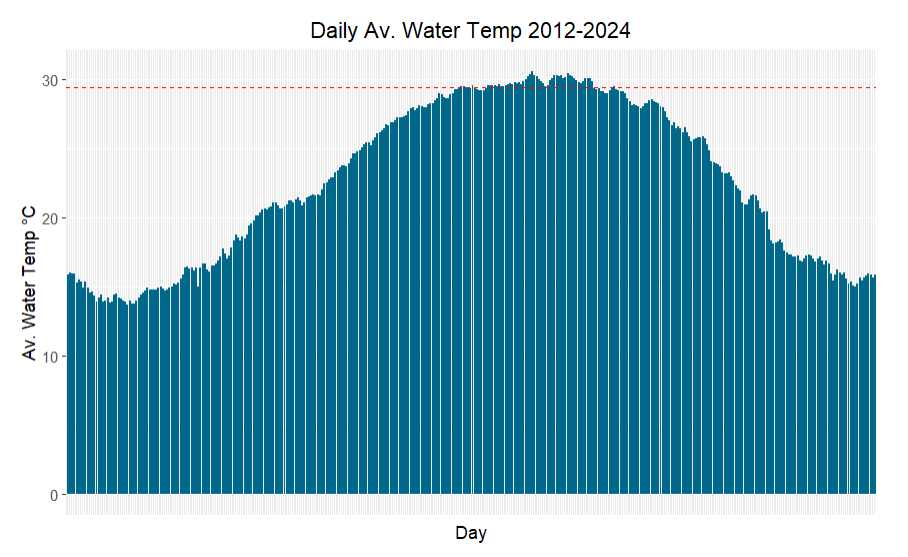
\includegraphics[keepaspectratio]{images/Screenshot 2025-04-18 194756.png}}

According to the U.S. Energy Information Administration, 33\% of the
electricity used in Alabama in 2023 was generated by the two nuclear
power plants in the state ({``U.s. Energy Information Administration -
EIA - Independent Statistics and Analysis''} 2024). Just one of the two
operating at half capacity would have a detrimental effect on consumer
energy use in the state. Residents would have to operate without
certainty of when they'd have power, fearful of outages and relying on
generators during the summer months. Essential businesses such as
hospitals, grocery stores, and pharmacies will take precedent, likely
not losing power completely, but possibly having to cut down on
electrical usage.

Throughout the data collection process, we did our best to reduce any
potential error. Despite using more than a decade of data collected by
the NOAA finding more data that goes back even further would be helpful
in making our results more accurate. We may not get a complete picture
of trends in water temperature, so we may not be able to make
predictions about the future as accurately. In the data we collected,
every day of each year has multiple observations throughout the day, so
we don't have to worry about only observing a maximum or minimum
temperature for that day. It is also important to note that we combined
a few data sets to create our final combined set. All but one year of
data came from the Dauphin Island 1 and 2 meteorological stations, which
are conveniently located less than a mile away from each other. This
difference would likely be negligible and can be ignored. Unfortunately,
the data for 2021 was missing or largely incomplete for every NOAA
station within 20 miles of Dauphin Island, so we had to use data from an
offshore station about 30 ESE of the other Dauphin Island stations. This
data may be different than what was actually observed at Dauphin Island,
so it is important to note that our results may be influenced. We'd much
prefer statistics from Dauphin Island itself in the year 2021, so our
data analysis can be rerun if it is ever uncovered.

It may also be useful to our analysis finding exact data on electricity
output and usage over the last decade or more in Alabama. For the
purposes of this paper, we did not find it to be necessary that we use
exact data. Instead, we cited data from the United States Energy
Information Administration and the World Nuclear Association to make
claims and analyses.

We can connect the data we've collected to previous studies to help
build a better understanding of water temperature in cooling nuclear
reactors. In an article about Climate Resilience, Matthew Bandyk states
the Oyster Creek nuclear power plant was closed, ``rather than spend
\$800 million developing a new water cooing system in order to reduce
the amount of heated water the plant discharged into the local bay. . .
harming the aquatic ecosystem'' (Bandyk 2020). If water temperatures
become too consistently high, it's possible the Dauphin Island plant may
have a future similar to the Oyster Creek plant. The article doesn't
just focus on one power plant though. They found there to be 17 cases in
which a nuclear power plant in the United States had to reduce
operations due to high water temperature in 2019. That number increased
to 25 cases in 2020. Bandyk mentions though, that the trend is not
linear, and can fluctuate based on yearly weather patterns like El Nino.
This data signals shutdowns due to extreme heat are not as rare as they
may initially seem.

This use of water to cool nuclear power plants is not just exclusive to
Dauphin Island, Alabama, or even the United States. Worldwide, this same
system is used. Different countries or regions may have different
guidelines on ideal water temperature, but the idea and consequences are
the same. For example, the World Nuclear Association writes about the
Brown's Ferry Nuclear Power Plant in Northern Alabama, ``In mid 2010,
TVA had to reduce power at its three Brown's Ferry Units in Alabama to
50\% in order to keep river water temperatures below 32 degrees C, at a
cost to some \$50 million to customers'' ({``Cooling Power Plants -
World Nuclear Association,''} n.d.). Worldwide, almost 10\% of all
energy used comes from the 440 nuclear power plants across the globe
({``Nuclear Power in the World Today - World Nuclear Association,''}
n.d.). The World Nuclear Association states that some countries like
France, Hungary, or Ukraine, rely on nuclear energy for more than half
of their electricity. In these cases, the threat of operating at half
capacity is more daunting, as it can effect much of a country's power
output.

Despite the research we've done on the topic, there are multiple
opportunities to build on the knowledge we've gained. Using local and
national guidelines, one can research the probability of partial
shutdowns at any nuclear power plant across the world. It may be
particularly helpful to research France's nuclear power plants as they
supply over 70\% of the country's electrical output. A major heat wave
and increase in surrounding water temperatures could lead to ruinous
power outages across the country. Researching the probability of these
outages and the effects they could have is a great first step to
mitigating a country-wide disaster.

Due to increasing concern for the effects of climate change on
environments, we would also recommend further research be done on how
the Dauphin Island power plant may be effected. If water temperature is
increasing on average year-over-year, the power plant could be at risk
for longer periods of working at 50\% capacity, further straining power
supplies in Alabama. Prevention and alleviation tactics would be the
best focuses of future study.

Finally, alternative water sources or water cooling systems could help
ease the stress on nuclear power plants. The use of groundwater is an
intriguing topic, but its slow replenishment could lead to future
resource issues. Rapid cooling of sea water is another interesting idea,
but trade offs must be studied to find the feasibility of this idea.
Upgrading existing cooling features like building a secondary cooling
tower to make the process more efficient should be looked into as well.

\bookmarksetup{startatroot}

\chapter*{References}\label{references}
\addcontentsline{toc}{chapter}{References}

\markboth{References}{References}

\phantomsection\label{refs}
\begin{CSLReferences}{1}{0}
\bibitem[\citeproctext]{ref-Bandyk2020}
Bandyk, Matthew. 2020. {``For Nuclear Plants Operating on Thin Margins,
Growing Climate Risks Prompt Tough Choices \textbar{} Utility Dive.''}
\url{https://www.utilitydive.com/news/for-nuclear-plants-operating-on-thin-margins-growing-climate-risks-prompt/584883/}.

\bibitem[\citeproctext]{ref-Cooling2020}
{``Cooling Power Plants - World Nuclear Association.''} n.d.
\url{https://world-nuclear.org/information-library/current-and-future-generation/cooling-power-plants}.

\bibitem[\citeproctext]{ref-electric}
{``Electricity Data Browser - Net Generation for All Sectors.''} 2024.
\url{https://www.eia.gov/electricity/data/browser/}.

\bibitem[\citeproctext]{ref-knuth84}
Knuth, Donald E. 1984. {``Literate Programming.''} \emph{Comput. J.} 27
(2): 97--111. \url{https://doi.org/10.1093/comjnl/27.2.97}.

\bibitem[\citeproctext]{ref-nceicoaa}
{``NCEI Coastal Water Temperature Guide - All Coastal Regions Table.''}
2025.
\url{https://www.ncei.noaa.gov/access/coastal-water-temperature-guide/all_table.html}.

\bibitem[\citeproctext]{ref-WNA2025}
{``Nuclear Power in the World Today - World Nuclear Association.''} n.d.
\url{https://world-nuclear.org/information-library/current-and-future-generation/nuclear-power-in-the-world-today}.

\bibitem[\citeproctext]{ref-portugal-pereira2024}
Portugal-Pereira, Joana, Miguel Esteban, and Kathleen Araújo. 2024.
{``Exposure of Future Nuclear Energy Infrastructure to Climate Change
Hazards: A Review Assessment.''} \emph{Energy Strategy Reviews} 53
(May): 101365. \url{https://doi.org/10.1016/j.esr.2024.101365}.

\bibitem[\citeproctext]{ref-EIA}
{``U.s. Energy Information Administration - EIA - Independent Statistics
and Analysis.''} 2024. \url{https://www.eia.gov/state/analysis.php}.

\end{CSLReferences}

\cleardoublepage
\phantomsection
\addcontentsline{toc}{part}{Appendices}
\appendix

\chapter{Draft: Data Documentation}\label{draft-data-documentation}

\subsection{Source 1}\label{source-1}

\#https://www.ncei.noaa.gov/access/coastal-water-temperature-guide/all\_table.html\#
This gives average monthly temperature of the water off Dauphin island.
There are \emph{Information Quality} and \emph{Disclaimer} tabs at the
bottom of the page, although the \emph{Disclaimer} tab doesn't say
anything of importance. Information Quality says that the data has to
follow guidelines from a Treasury and General Government Appropriations
act for fair and accurate reporting. The data would be used to evaluate
the likelihood of water temps reaching the 85 degree threshold in
different months. Unfortunately, it doesn't have daily data, so we'd
look elsewhere for that. (\textbf{nceicoa?})

\#read fwf to fix the data we read in\#
https://www.ndbc.noaa.gov/obs.shtml Click on link to get to map. Click
on view history. Then can download any data wanted dpha12024.txt. This
site has real data every half hour for all of 2024 that comes directly
from the Dauphin Island site. There's also data from 2021-2023, and from
January of 2025. I would want to use this data like I said above,
finding the likelihood of water temps reaching 85 degrees (or 29.44
degrees Celcius). (\textbf{nceicoa?})

\begin{Shaded}
\begin{Highlighting}[]
\FunctionTok{setwd}\NormalTok{(}\StringTok{"C:/Users/Dominic Sander/Downloads/Stat 349"}\NormalTok{)}
\FunctionTok{library}\NormalTok{(readr)}
\NormalTok{dpha2h2012 }\OtherTok{\textless{}{-}} \FunctionTok{read\_table}\NormalTok{(}\StringTok{"dpha1h2012.txt"}\NormalTok{)}
\end{Highlighting}
\end{Shaded}

\begin{verbatim}

-- Column specification --------------------------------------------------------
cols(
  `#YY` = col_character(),
  MM = col_character(),
  DD = col_character(),
  hh = col_character(),
  mm = col_character(),
  DEPTH = col_character(),
  OTMP = col_character(),
  COND = col_character(),
  SAL = col_character(),
  `O2%` = col_character(),
  O2PPM = col_character(),
  CLCON = col_character(),
  TURB = col_character(),
  PH = col_character(),
  EH = col_character()
)
\end{verbatim}

\begin{Shaded}
\begin{Highlighting}[]
\NormalTok{dpha2h2013 }\OtherTok{\textless{}{-}} \FunctionTok{read\_table}\NormalTok{(}\StringTok{"dpah1h2013.txt"}\NormalTok{)}
\end{Highlighting}
\end{Shaded}

\begin{verbatim}

-- Column specification --------------------------------------------------------
cols(
  `#YY` = col_character(),
  MM = col_character(),
  DD = col_character(),
  hh = col_character(),
  mm = col_character(),
  DEPTH = col_character(),
  OTMP = col_character(),
  COND = col_character(),
  SAL = col_character(),
  `O2%` = col_character(),
  O2PPM = col_character(),
  CLCON = col_character(),
  TURB = col_character(),
  PH = col_character(),
  EH = col_character()
)
\end{verbatim}

\begin{Shaded}
\begin{Highlighting}[]
\NormalTok{dpha2h2014 }\OtherTok{\textless{}{-}} \FunctionTok{read\_table}\NormalTok{(}\StringTok{"dpha1h2014.txt"}\NormalTok{)}
\end{Highlighting}
\end{Shaded}

\begin{verbatim}

-- Column specification --------------------------------------------------------
cols(
  `#YY` = col_character(),
  MM = col_character(),
  DD = col_character(),
  hh = col_character(),
  mm = col_character(),
  DEPTH = col_character(),
  OTMP = col_character(),
  COND = col_character(),
  SAL = col_character(),
  `O2%` = col_character(),
  O2PPM = col_character(),
  CLCON = col_character(),
  TURB = col_character(),
  PH = col_character(),
  EH = col_character()
)
\end{verbatim}

\begin{Shaded}
\begin{Highlighting}[]
\NormalTok{dpha2h2015 }\OtherTok{\textless{}{-}} \FunctionTok{read\_table}\NormalTok{(}\StringTok{"dpha1h2105.txt"}\NormalTok{)}
\end{Highlighting}
\end{Shaded}

\begin{verbatim}

-- Column specification --------------------------------------------------------
cols(
  `#YY` = col_character(),
  MM = col_character(),
  DD = col_character(),
  hh = col_character(),
  mm = col_character(),
  DEPTH = col_character(),
  OTMP = col_character(),
  COND = col_character(),
  SAL = col_character(),
  `O2%` = col_character(),
  O2PPM = col_character(),
  CLCON = col_character(),
  TURB = col_character(),
  PH = col_character(),
  EH = col_character()
)
\end{verbatim}

\begin{Shaded}
\begin{Highlighting}[]
\NormalTok{dpha2h2016 }\OtherTok{\textless{}{-}} \FunctionTok{read\_table}\NormalTok{(}\StringTok{"dpha2h2016.txt"}\NormalTok{)}
\end{Highlighting}
\end{Shaded}

\begin{verbatim}

-- Column specification --------------------------------------------------------
cols(
  `#YY` = col_character(),
  MM = col_character(),
  DD = col_character(),
  hh = col_character(),
  mm = col_character(),
  DEPTH = col_character(),
  OTMP = col_character(),
  COND = col_character(),
  SAL = col_character(),
  `O2%` = col_character(),
  O2PPM = col_character(),
  CLCON = col_character(),
  TURB = col_character(),
  PH = col_character(),
  EH = col_character()
)
\end{verbatim}

\begin{Shaded}
\begin{Highlighting}[]
\NormalTok{dpha2h2017 }\OtherTok{\textless{}{-}} \FunctionTok{read\_table}\NormalTok{(}\StringTok{"dpha2h2017.txt"}\NormalTok{)}
\end{Highlighting}
\end{Shaded}

\begin{verbatim}

-- Column specification --------------------------------------------------------
cols(
  `#YY` = col_character(),
  MM = col_character(),
  DD = col_character(),
  hh = col_character(),
  mm = col_character(),
  DEPTH = col_character(),
  OTMP = col_character(),
  COND = col_character(),
  SAL = col_character(),
  `O2%` = col_character(),
  O2PPM = col_character(),
  CLCON = col_character(),
  TURB = col_character(),
  PH = col_character(),
  EH = col_character()
)
\end{verbatim}

\begin{Shaded}
\begin{Highlighting}[]
\NormalTok{dpha2h2018 }\OtherTok{\textless{}{-}} \FunctionTok{read\_table}\NormalTok{(}\StringTok{"dpha2h2018.txt"}\NormalTok{)}
\end{Highlighting}
\end{Shaded}

\begin{verbatim}

-- Column specification --------------------------------------------------------
cols(
  `#YY` = col_character(),
  MM = col_character(),
  DD = col_character(),
  hh = col_character(),
  mm = col_character(),
  DEPTH = col_character(),
  OTMP = col_character(),
  COND = col_character(),
  SAL = col_character(),
  `O2%` = col_character(),
  O2PPM = col_character(),
  CLCON = col_character(),
  TURB = col_character(),
  PH = col_character(),
  EH = col_character()
)
\end{verbatim}

\begin{Shaded}
\begin{Highlighting}[]
\NormalTok{dpha2h2019 }\OtherTok{\textless{}{-}} \FunctionTok{read\_table}\NormalTok{(}\StringTok{"dpha2h2019.txt"}\NormalTok{)}
\end{Highlighting}
\end{Shaded}

\begin{verbatim}

-- Column specification --------------------------------------------------------
cols(
  `#YY` = col_character(),
  MM = col_character(),
  DD = col_character(),
  hh = col_character(),
  mm = col_character(),
  DEPTH = col_character(),
  OTMP = col_character(),
  COND = col_character(),
  SAL = col_character(),
  `O2%` = col_character(),
  O2PPM = col_character(),
  CLCON = col_character(),
  TURB = col_character(),
  PH = col_character(),
  EH = col_character()
)
\end{verbatim}

\begin{Shaded}
\begin{Highlighting}[]
\NormalTok{dpha2h2020 }\OtherTok{\textless{}{-}} \FunctionTok{read\_table}\NormalTok{(}\StringTok{"dpha2h2020.txt"}\NormalTok{)}
\end{Highlighting}
\end{Shaded}

\begin{verbatim}

-- Column specification --------------------------------------------------------
cols(
  `#YY` = col_character(),
  MM = col_character(),
  DD = col_character(),
  hh = col_character(),
  mm = col_character(),
  DEPTH = col_character(),
  OTMP = col_character(),
  COND = col_character(),
  SAL = col_character(),
  `O2%` = col_character(),
  O2PPM = col_character(),
  CLCON = col_character(),
  TURB = col_character(),
  PH = col_character(),
  EH = col_character()
)
\end{verbatim}

\begin{Shaded}
\begin{Highlighting}[]
\NormalTok{X42012h2021 }\OtherTok{\textless{}{-}} \FunctionTok{read\_table}\NormalTok{(}\StringTok{"42012h2021.txt"}\NormalTok{)}
\end{Highlighting}
\end{Shaded}

\begin{verbatim}

-- Column specification --------------------------------------------------------
cols(
  `#YY` = col_character(),
  MM = col_character(),
  DD = col_character(),
  hh = col_character(),
  mm = col_character(),
  WDIR = col_character(),
  WSPD = col_character(),
  GST = col_character(),
  WVHT = col_character(),
  DPD = col_character(),
  APD = col_character(),
  MWD = col_character(),
  PRES = col_character(),
  ATMP = col_character(),
  WTMP = col_character(),
  DEWP = col_character(),
  VIS = col_character(),
  TIDE = col_character()
)
\end{verbatim}

\begin{verbatim}
Warning: 51483 parsing failures.
row col   expected     actual             file
  2  -- 18 columns 19 columns '42012h2021.txt'
  3  -- 18 columns 19 columns '42012h2021.txt'
  4  -- 18 columns 19 columns '42012h2021.txt'
  5  -- 18 columns 19 columns '42012h2021.txt'
  6  -- 18 columns 19 columns '42012h2021.txt'
... ... .......... .......... ................
See problems(...) for more details.
\end{verbatim}

\begin{Shaded}
\begin{Highlighting}[]
\NormalTok{dpha2h2022 }\OtherTok{\textless{}{-}} \FunctionTok{read\_table}\NormalTok{(}\StringTok{"dpha2h2022.txt"}\NormalTok{)}
\end{Highlighting}
\end{Shaded}

\begin{verbatim}

-- Column specification --------------------------------------------------------
cols(
  `#YY` = col_character(),
  MM = col_character(),
  DD = col_character(),
  hh = col_character(),
  mm = col_character(),
  WDIR = col_character(),
  WSPD = col_character(),
  GST = col_character(),
  WVHT = col_character(),
  DPD = col_character(),
  APD = col_character(),
  MWD = col_character(),
  PRES = col_character(),
  ATMP = col_character(),
  WTMP = col_character(),
  DEWP = col_character(),
  VIS = col_character(),
  TIDE = col_character()
)
\end{verbatim}

\begin{Shaded}
\begin{Highlighting}[]
\NormalTok{dpha2h2023 }\OtherTok{\textless{}{-}} \FunctionTok{read\_table}\NormalTok{(}\StringTok{"dpha2h2023.txt"}\NormalTok{)}
\end{Highlighting}
\end{Shaded}

\begin{verbatim}

-- Column specification --------------------------------------------------------
cols(
  `#YY` = col_character(),
  MM = col_character(),
  DD = col_character(),
  hh = col_character(),
  mm = col_character(),
  WDIR = col_character(),
  WSPD = col_character(),
  GST = col_character(),
  WVHT = col_character(),
  DPD = col_character(),
  APD = col_character(),
  MWD = col_character(),
  PRES = col_character(),
  ATMP = col_character(),
  WTMP = col_character(),
  DEWP = col_character(),
  VIS = col_character(),
  TIDE = col_character()
)
\end{verbatim}

\begin{Shaded}
\begin{Highlighting}[]
\NormalTok{dpha2h2024 }\OtherTok{\textless{}{-}} \FunctionTok{read\_table}\NormalTok{(}\StringTok{"dpha2h2024.txt"}\NormalTok{)}
\end{Highlighting}
\end{Shaded}

\begin{verbatim}

-- Column specification --------------------------------------------------------
cols(
  `#YY` = col_character(),
  MM = col_character(),
  DD = col_character(),
  hh = col_character(),
  mm = col_character(),
  WDIR = col_character(),
  WSPD = col_character(),
  GST = col_character(),
  WVHT = col_character(),
  DPD = col_character(),
  APD = col_character(),
  MWD = col_character(),
  PRES = col_character(),
  ATMP = col_character(),
  WTMP = col_character(),
  DEWP = col_character(),
  VIS = col_character(),
  TIDE = col_character()
)
\end{verbatim}

\begin{Shaded}
\begin{Highlighting}[]
\FunctionTok{library}\NormalTok{(dplyr)}
\end{Highlighting}
\end{Shaded}

\begin{verbatim}

Attaching package: 'dplyr'
\end{verbatim}

\begin{verbatim}
The following objects are masked from 'package:stats':

    filter, lag
\end{verbatim}

\begin{verbatim}
The following objects are masked from 'package:base':

    intersect, setdiff, setequal, union
\end{verbatim}

\begin{Shaded}
\begin{Highlighting}[]
\FunctionTok{library}\NormalTok{(tidyr)}
\FunctionTok{library}\NormalTok{(ggplot2)}
\FunctionTok{library}\NormalTok{(knitr)}
\end{Highlighting}
\end{Shaded}

\begin{verbatim}
Warning: package 'knitr' was built under R version 4.3.3
\end{verbatim}

\begin{Shaded}
\begin{Highlighting}[]
\NormalTok{dpha2\_12 }\OtherTok{\textless{}{-}}\NormalTok{ dpha2h2012 }\SpecialCharTok{\%\textgreater{}\%} \FunctionTok{select}\NormalTok{(}\StringTok{"\#YY"}\NormalTok{,}\StringTok{"MM"}\NormalTok{,}\StringTok{"DD"}\NormalTok{,}\StringTok{"hh"}\NormalTok{,}\StringTok{"mm"}\NormalTok{,}\StringTok{"OTMP"}\NormalTok{) }\SpecialCharTok{\%\textgreater{}\%}
   \FunctionTok{rename}\NormalTok{(}\AttributeTok{WTMP=}\NormalTok{OTMP)}
\NormalTok{dpha2\_12 }\OtherTok{\textless{}{-}}\NormalTok{ dpha2\_12[}\SpecialCharTok{{-}}\DecValTok{1}\NormalTok{, ]}

\NormalTok{dpha2\_13 }\OtherTok{\textless{}{-}}\NormalTok{ dpha2h2013 }\SpecialCharTok{\%\textgreater{}\%} \FunctionTok{select}\NormalTok{(}\StringTok{"\#YY"}\NormalTok{,}\StringTok{"MM"}\NormalTok{,}\StringTok{"DD"}\NormalTok{,}\StringTok{"hh"}\NormalTok{,}\StringTok{"mm"}\NormalTok{,}\StringTok{"OTMP"}\NormalTok{) }\SpecialCharTok{\%\textgreater{}\%}
   \FunctionTok{rename}\NormalTok{(}\AttributeTok{WTMP=}\NormalTok{OTMP)}
\NormalTok{dpha2\_13 }\OtherTok{\textless{}{-}}\NormalTok{ dpha2\_13[}\SpecialCharTok{{-}}\DecValTok{1}\NormalTok{, ]}

\NormalTok{dpha2\_14 }\OtherTok{\textless{}{-}}\NormalTok{ dpha2h2014 }\SpecialCharTok{\%\textgreater{}\%} \FunctionTok{select}\NormalTok{(}\StringTok{"\#YY"}\NormalTok{,}\StringTok{"MM"}\NormalTok{,}\StringTok{"DD"}\NormalTok{,}\StringTok{"hh"}\NormalTok{,}\StringTok{"mm"}\NormalTok{,}\StringTok{"OTMP"}\NormalTok{) }\SpecialCharTok{\%\textgreater{}\%}
   \FunctionTok{rename}\NormalTok{(}\AttributeTok{WTMP=}\NormalTok{OTMP)}
\NormalTok{dpha2\_14 }\OtherTok{\textless{}{-}}\NormalTok{ dpha2\_14[}\SpecialCharTok{{-}}\DecValTok{1}\NormalTok{, ]}

\NormalTok{dpha2\_15 }\OtherTok{\textless{}{-}}\NormalTok{ dpha2h2015 }\SpecialCharTok{\%\textgreater{}\%} \FunctionTok{select}\NormalTok{(}\StringTok{"\#YY"}\NormalTok{,}\StringTok{"MM"}\NormalTok{,}\StringTok{"DD"}\NormalTok{,}\StringTok{"hh"}\NormalTok{,}\StringTok{"mm"}\NormalTok{,}\StringTok{"OTMP"}\NormalTok{) }\SpecialCharTok{\%\textgreater{}\%}
   \FunctionTok{rename}\NormalTok{(}\AttributeTok{WTMP=}\NormalTok{OTMP)}
\NormalTok{dpha2\_15 }\OtherTok{\textless{}{-}}\NormalTok{ dpha2\_15[}\SpecialCharTok{{-}}\DecValTok{1}\NormalTok{, ]}

\NormalTok{dpha2\_16 }\OtherTok{\textless{}{-}}\NormalTok{ dpha2h2016 }\SpecialCharTok{\%\textgreater{}\%} \FunctionTok{select}\NormalTok{(}\StringTok{"\#YY"}\NormalTok{,}\StringTok{"MM"}\NormalTok{,}\StringTok{"DD"}\NormalTok{,}\StringTok{"hh"}\NormalTok{,}\StringTok{"mm"}\NormalTok{,}\StringTok{"OTMP"}\NormalTok{) }\SpecialCharTok{\%\textgreater{}\%}
   \FunctionTok{rename}\NormalTok{(}\AttributeTok{WTMP=}\NormalTok{OTMP)}
\NormalTok{dpha2\_16 }\OtherTok{\textless{}{-}}\NormalTok{ dpha2\_16[}\SpecialCharTok{{-}}\DecValTok{1}\NormalTok{, ] }

\NormalTok{dpha2\_17 }\OtherTok{\textless{}{-}}\NormalTok{ dpha2h2017 }\SpecialCharTok{\%\textgreater{}\%} \FunctionTok{select}\NormalTok{(}\StringTok{"\#YY"}\NormalTok{,}\StringTok{"MM"}\NormalTok{,}\StringTok{"DD"}\NormalTok{,}\StringTok{"hh"}\NormalTok{,}\StringTok{"mm"}\NormalTok{,}\StringTok{"OTMP"}\NormalTok{) }\SpecialCharTok{\%\textgreater{}\%}
  \FunctionTok{rename}\NormalTok{(}\AttributeTok{WTMP=}\NormalTok{OTMP)}
\NormalTok{dpha2\_17 }\OtherTok{\textless{}{-}}\NormalTok{ dpha2\_17[}\SpecialCharTok{{-}}\DecValTok{1}\NormalTok{, ]}

\NormalTok{dpha2\_18 }\OtherTok{\textless{}{-}}\NormalTok{ dpha2h2018 }\SpecialCharTok{\%\textgreater{}\%} \FunctionTok{select}\NormalTok{(}\StringTok{"\#YY"}\NormalTok{,}\StringTok{"MM"}\NormalTok{,}\StringTok{"DD"}\NormalTok{,}\StringTok{"hh"}\NormalTok{,}\StringTok{"mm"}\NormalTok{,}\StringTok{"OTMP"}\NormalTok{) }\SpecialCharTok{\%\textgreater{}\%}
  \FunctionTok{rename}\NormalTok{(}\AttributeTok{WTMP=}\NormalTok{OTMP)}
\NormalTok{dpha2\_18 }\OtherTok{\textless{}{-}}\NormalTok{ dpha2\_18[}\SpecialCharTok{{-}}\DecValTok{1}\NormalTok{, ]}

\NormalTok{dpha2\_19 }\OtherTok{\textless{}{-}}\NormalTok{ dpha2h2019 }\SpecialCharTok{\%\textgreater{}\%} \FunctionTok{select}\NormalTok{(}\StringTok{"\#YY"}\NormalTok{,}\StringTok{"MM"}\NormalTok{,}\StringTok{"DD"}\NormalTok{,}\StringTok{"hh"}\NormalTok{,}\StringTok{"mm"}\NormalTok{,}\StringTok{"OTMP"}\NormalTok{) }\SpecialCharTok{\%\textgreater{}\%}
  \FunctionTok{rename}\NormalTok{(}\AttributeTok{WTMP=}\NormalTok{OTMP)}
\NormalTok{dpha2\_19 }\OtherTok{\textless{}{-}}\NormalTok{ dpha2\_19[}\SpecialCharTok{{-}}\DecValTok{1}\NormalTok{, ]}

\NormalTok{dpha2\_20 }\OtherTok{\textless{}{-}}\NormalTok{ dpha2h2020 }\SpecialCharTok{\%\textgreater{}\%} \FunctionTok{select}\NormalTok{(}\StringTok{"\#YY"}\NormalTok{,}\StringTok{"MM"}\NormalTok{,}\StringTok{"DD"}\NormalTok{,}\StringTok{"hh"}\NormalTok{,}\StringTok{"mm"}\NormalTok{,}\StringTok{"OTMP"}\NormalTok{) }\SpecialCharTok{\%\textgreater{}\%}
  \FunctionTok{rename}\NormalTok{(}\AttributeTok{WTMP=}\NormalTok{OTMP)}
\NormalTok{dpha2\_20 }\OtherTok{\textless{}{-}}\NormalTok{ dpha2\_20[}\SpecialCharTok{{-}}\DecValTok{1}\NormalTok{, ]}

\NormalTok{X42012h\_21 }\OtherTok{\textless{}{-}}\NormalTok{ X42012h2021 }\SpecialCharTok{\%\textgreater{}\%} \FunctionTok{select}\NormalTok{(}\StringTok{"\#YY"}\NormalTok{,}\StringTok{"MM"}\NormalTok{,}\StringTok{"DD"}\NormalTok{,}\StringTok{"hh"}\NormalTok{,}\StringTok{"mm"}\NormalTok{,}\StringTok{"WTMP"}\NormalTok{)}
\NormalTok{X42012h\_21 }\OtherTok{\textless{}{-}}\NormalTok{ X42012h\_21[}\SpecialCharTok{{-}}\DecValTok{1}\NormalTok{, ]}

\NormalTok{dpha2\_22 }\OtherTok{\textless{}{-}}\NormalTok{ dpha2h2022 }\SpecialCharTok{\%\textgreater{}\%} \FunctionTok{select}\NormalTok{(}\StringTok{"\#YY"}\NormalTok{,}\StringTok{"MM"}\NormalTok{,}\StringTok{"DD"}\NormalTok{,}\StringTok{"hh"}\NormalTok{,}\StringTok{"mm"}\NormalTok{,}\StringTok{"WTMP"}\NormalTok{) }
\NormalTok{dpha2\_22 }\OtherTok{\textless{}{-}}\NormalTok{ dpha2\_22[}\SpecialCharTok{{-}}\DecValTok{1}\NormalTok{, ]}
\NormalTok{dpha2\_23 }\OtherTok{\textless{}{-}}\NormalTok{ dpha2h2023 }\SpecialCharTok{\%\textgreater{}\%} \FunctionTok{select}\NormalTok{(}\StringTok{"\#YY"}\NormalTok{,}\StringTok{"MM"}\NormalTok{,}\StringTok{"DD"}\NormalTok{,}\StringTok{"hh"}\NormalTok{,}\StringTok{"mm"}\NormalTok{,}\StringTok{"WTMP"}\NormalTok{) }
\NormalTok{dpha2\_23 }\OtherTok{\textless{}{-}}\NormalTok{ dpha2\_23[}\SpecialCharTok{{-}}\DecValTok{1}\NormalTok{, ]}
\NormalTok{dpha2\_24 }\OtherTok{\textless{}{-}}\NormalTok{ dpha2h2024 }\SpecialCharTok{\%\textgreater{}\%} \FunctionTok{select}\NormalTok{(}\StringTok{"\#YY"}\NormalTok{,}\StringTok{"MM"}\NormalTok{,}\StringTok{"DD"}\NormalTok{,}\StringTok{"hh"}\NormalTok{,}\StringTok{"mm"}\NormalTok{,}\StringTok{"WTMP"}\NormalTok{) }
\NormalTok{dpha2\_24 }\OtherTok{\textless{}{-}}\NormalTok{ dpha2\_24[}\SpecialCharTok{{-}}\DecValTok{1}\NormalTok{, ]}

\NormalTok{dpha\_combined }\OtherTok{\textless{}{-}} \FunctionTok{bind\_rows}\NormalTok{(dpha2\_12, dpha2\_13, dpha2\_14, dpha2\_15, dpha2\_16, dpha2\_17, dpha2\_18, dpha2\_19, dpha2\_20, X42012h\_21, dpha2\_22, dpha2\_23, dpha2\_24}
\NormalTok{) }\SpecialCharTok{\%\textgreater{}\%}
  \FunctionTok{arrange}\NormalTok{(}\StringTok{\textasciigrave{}}\AttributeTok{\#YY}\StringTok{\textasciigrave{}}\NormalTok{, MM, DD, hh, mm) }\SpecialCharTok{\%\textgreater{}\%}
  \FunctionTok{filter}\NormalTok{(WTMP }\SpecialCharTok{\textless{}=}\DecValTok{40}\NormalTok{)}
\end{Highlighting}
\end{Shaded}

Create dataset for av temp

\begin{Shaded}
\begin{Highlighting}[]
\NormalTok{dpha\_av }\OtherTok{\textless{}{-}}\NormalTok{ dpha\_combined }\SpecialCharTok{\%\textgreater{}\%}
  \FunctionTok{mutate}\NormalTok{(}\AttributeTok{WTMP =} \FunctionTok{as.numeric}\NormalTok{(WTMP)) }\SpecialCharTok{\%\textgreater{}\%}
  \FunctionTok{filter}\NormalTok{(WTMP }\SpecialCharTok{\textless{}=}\DecValTok{40}\NormalTok{) }\SpecialCharTok{\%\textgreater{}\%}
  \FunctionTok{group\_by}\NormalTok{(}\StringTok{\textquotesingle{}\#YY\textquotesingle{}}\NormalTok{, MM, DD) }\SpecialCharTok{\%\textgreater{}\%}
  \FunctionTok{summarize}\NormalTok{(}\AttributeTok{Avg\_WTMP =} \FunctionTok{mean}\NormalTok{(WTMP, }\AttributeTok{na.rm =} \ConstantTok{TRUE}\NormalTok{), }\AttributeTok{.groups =} \StringTok{"drop"}\NormalTok{)}

\NormalTok{dpha\_over85 }\OtherTok{\textless{}{-}}\NormalTok{ dpha\_av }\SpecialCharTok{\%\textgreater{}\%}
  \FunctionTok{filter}\NormalTok{(Avg\_WTMP}\SpecialCharTok{\textgreater{}=}\FloatTok{29.4444}\NormalTok{)}
\end{Highlighting}
\end{Shaded}

Graph of av. temp by day

\begin{Shaded}
\begin{Highlighting}[]
\FunctionTok{colnames}\NormalTok{(dpha\_av)}
\end{Highlighting}
\end{Shaded}

\begin{verbatim}
[1] "\"#YY\""  "MM"       "DD"       "Avg_WTMP"
\end{verbatim}

\begin{Shaded}
\begin{Highlighting}[]
\NormalTok{dpha\_av }\OtherTok{\textless{}{-}}\NormalTok{ dpha\_av }\SpecialCharTok{\%\textgreater{}\%}
  \FunctionTok{select}\NormalTok{(}\SpecialCharTok{{-}}\StringTok{\textasciigrave{}}\SpecialCharTok{\textbackslash{}"}\AttributeTok{\#YY}\SpecialCharTok{\textbackslash{}"}\StringTok{\textasciigrave{}}\NormalTok{)}

\FunctionTok{ggplot}\NormalTok{(dpha\_av, }\FunctionTok{aes}\NormalTok{(}\AttributeTok{x =} \FunctionTok{factor}\NormalTok{(}\FunctionTok{paste}\NormalTok{(MM, DD, }\AttributeTok{sep =} \StringTok{"{-}"}\NormalTok{)), }\AttributeTok{y =}\NormalTok{ Avg\_WTMP)) }\SpecialCharTok{+}
  \FunctionTok{geom\_bar}\NormalTok{(}\AttributeTok{stat =} \StringTok{"identity"}\NormalTok{, }\AttributeTok{fill =} \StringTok{"deepskyblue4"}\NormalTok{) }\SpecialCharTok{+} 
  \FunctionTok{geom\_hline}\NormalTok{(}\AttributeTok{yintercept =} \FloatTok{29.44}\NormalTok{, }\AttributeTok{linetype =} \StringTok{"dashed"}\NormalTok{, }\AttributeTok{color =} \StringTok{"red"}\NormalTok{) }\SpecialCharTok{+}
  \FunctionTok{labs}\NormalTok{(}\AttributeTok{x =} \StringTok{"Day"}\NormalTok{, }\AttributeTok{y =} \StringTok{"Av. Water Temp °C"}\NormalTok{, }\AttributeTok{title =} \StringTok{"Daily Av. Water Temp 2012{-}2024"}\NormalTok{) }\SpecialCharTok{+}
  \FunctionTok{theme}\NormalTok{(}\AttributeTok{axis.text.x =} \FunctionTok{element\_blank}\NormalTok{(),  }
        \AttributeTok{axis.ticks.x =} \FunctionTok{element\_blank}\NormalTok{(), }
        \AttributeTok{plot.title =} \FunctionTok{element\_text}\NormalTok{(}\AttributeTok{hjust =} \FloatTok{0.5}\NormalTok{))}
\end{Highlighting}
\end{Shaded}

\pandocbounded{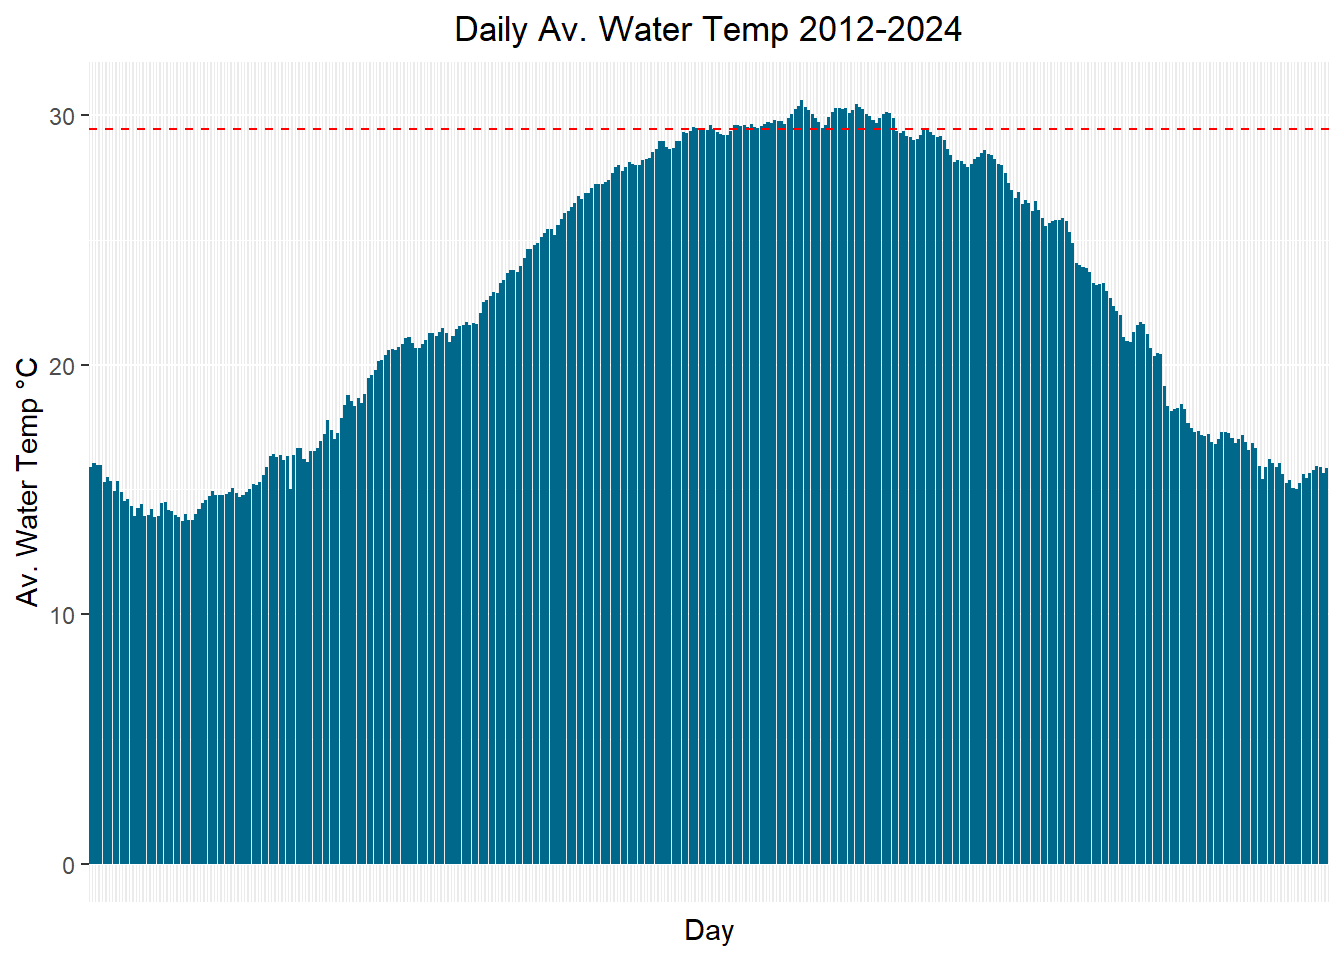
\includegraphics[keepaspectratio]{draft-data-doc_files/figure-pdf/unnamed-chunk-3-1.pdf}}

Total Days Per Month With Av. Over 29.44

\begin{Shaded}
\begin{Highlighting}[]
\NormalTok{month\_count }\OtherTok{\textless{}{-}}\NormalTok{ dpha\_over85 }\SpecialCharTok{\%\textgreater{}\%}
  \FunctionTok{group\_by}\NormalTok{(MM) }\SpecialCharTok{\%\textgreater{}\%}
  \FunctionTok{summarize}\NormalTok{(}\AttributeTok{Count=}\FunctionTok{n}\NormalTok{(), }\AttributeTok{.groups=}\StringTok{"drop"}\NormalTok{)}\SpecialCharTok{\%\textgreater{}\%}
  \FunctionTok{complete}\NormalTok{(}\AttributeTok{MM=}\FunctionTok{sprintf}\NormalTok{(}\StringTok{"\%02d"}\NormalTok{, }\DecValTok{1}\SpecialCharTok{:}\DecValTok{12}\NormalTok{), }\AttributeTok{fill =} \FunctionTok{list}\NormalTok{(}\AttributeTok{Count=}\DecValTok{0}\NormalTok{))}

\FunctionTok{data}\NormalTok{(month\_count)}
\end{Highlighting}
\end{Shaded}

\begin{verbatim}
Warning in data(month_count): data set 'month_count' not found
\end{verbatim}

\begin{Shaded}
\begin{Highlighting}[]
\FunctionTok{kable}\NormalTok{(month\_count)}
\end{Highlighting}
\end{Shaded}

\begin{longtable}[]{@{}lr@{}}
\toprule\noalign{}
MM & Count \\
\midrule\noalign{}
\endhead
\bottomrule\noalign{}
\endlastfoot
01 & 0 \\
02 & 0 \\
03 & 0 \\
04 & 0 \\
05 & 0 \\
06 & 2 \\
07 & 24 \\
08 & 25 \\
09 & 2 \\
10 & 0 \\
11 & 0 \\
12 & 0 \\
\end{longtable}

Total Days Per Month With Obs. \textgreater{} 29.44 in 2024

\begin{Shaded}
\begin{Highlighting}[]
\NormalTok{dpha2\_24\_29 }\OtherTok{\textless{}{-}}\NormalTok{ dpha2\_24 }\SpecialCharTok{\%\textgreater{}\%}
  \FunctionTok{filter}\NormalTok{(WTMP }\SpecialCharTok{\textgreater{}=} \FloatTok{29.44}\NormalTok{) }\SpecialCharTok{\%\textgreater{}\%}
  \FunctionTok{filter}\NormalTok{(WTMP }\SpecialCharTok{\textless{}=} \DecValTok{50}\NormalTok{)}

\NormalTok{month\_obs }\OtherTok{\textless{}{-}}\NormalTok{ dpha2\_24\_29 }\SpecialCharTok{\%\textgreater{}\%}
  \FunctionTok{group\_by}\NormalTok{(MM) }\SpecialCharTok{\%\textgreater{}\%}
  \FunctionTok{summarize}\NormalTok{(}\AttributeTok{Days =} \FunctionTok{n\_distinct}\NormalTok{(DD), }\AttributeTok{.groups =} \StringTok{"drop"}\NormalTok{)}

\FunctionTok{kable}\NormalTok{(month\_obs, }\AttributeTok{caption=}\StringTok{"Total Days Per Month With an Obs. \textgreater{} 29.44° C"}\NormalTok{, }\AttributeTok{col.names=}\FunctionTok{c}\NormalTok{(}\StringTok{"Month"}\NormalTok{, }\StringTok{"Total Days"}\NormalTok{))}
\end{Highlighting}
\end{Shaded}

\begin{longtable}[]{@{}lr@{}}
\caption{Total Days Per Month With an Obs. \textgreater{} 29.44°
C}\tabularnewline
\toprule\noalign{}
Month & Total Days \\
\midrule\noalign{}
\endfirsthead
\toprule\noalign{}
Month & Total Days \\
\midrule\noalign{}
\endhead
\bottomrule\noalign{}
\endlastfoot
05 & 7 \\
06 & 12 \\
07 & 31 \\
08 & 31 \\
09 & 13 \\
\end{longtable}

Total days per year with daily max temp above 29.44

\begin{Shaded}
\begin{Highlighting}[]
\FunctionTok{library}\NormalTok{(lubridate)}
\end{Highlighting}
\end{Shaded}

\begin{verbatim}
Warning: package 'lubridate' was built under R version 4.3.3
\end{verbatim}

\begin{verbatim}

Attaching package: 'lubridate'
\end{verbatim}

\begin{verbatim}
The following objects are masked from 'package:base':

    date, intersect, setdiff, union
\end{verbatim}

\begin{Shaded}
\begin{Highlighting}[]
\NormalTok{dpha\_combined }\OtherTok{\textless{}{-}}\NormalTok{ dpha\_combined }\SpecialCharTok{\%\textgreater{}\%}
  \FunctionTok{mutate}\NormalTok{(}
    \AttributeTok{Date =} \FunctionTok{make\_date}\NormalTok{(}\AttributeTok{year =} \FunctionTok{as.integer}\NormalTok{(}\StringTok{\textasciigrave{}}\AttributeTok{\#YY}\StringTok{\textasciigrave{}}\NormalTok{), }\AttributeTok{month =} \FunctionTok{as.integer}\NormalTok{(MM), }\AttributeTok{day =} \FunctionTok{as.integer}\NormalTok{(DD))}
\NormalTok{  )}

\NormalTok{year\_above\_29 }\OtherTok{\textless{}{-}}\NormalTok{ dpha\_combined }\SpecialCharTok{\%\textgreater{}\%}
  \FunctionTok{filter}\NormalTok{(WTMP }\SpecialCharTok{\textgreater{}=} \FloatTok{29.44}\NormalTok{, WTMP }\SpecialCharTok{\textless{}=} \DecValTok{50}\NormalTok{) }\SpecialCharTok{\%\textgreater{}\%}
  \FunctionTok{group\_by}\NormalTok{(}\AttributeTok{Year =} \FunctionTok{year}\NormalTok{(Date)) }\SpecialCharTok{\%\textgreater{}\%}
  \FunctionTok{summarise}\NormalTok{(}
    \AttributeTok{Days\_Above\_29\_44C =} \FunctionTok{n\_distinct}\NormalTok{(Date), }
    \AttributeTok{Max\_temp =} \FunctionTok{max}\NormalTok{(WTMP, }\AttributeTok{na.rm=}\ConstantTok{TRUE}\NormalTok{),}
    \AttributeTok{.groups =} \StringTok{"drop"}\NormalTok{,}
\NormalTok{    )}
\end{Highlighting}
\end{Shaded}

Predictive model for next five years

\begin{Shaded}
\begin{Highlighting}[]
\NormalTok{water\_model }\OtherTok{\textless{}{-}} \FunctionTok{lm}\NormalTok{(Days\_Above\_29\_44C }\SpecialCharTok{\textasciitilde{}}\NormalTok{ Year, }\AttributeTok{data =}\NormalTok{ year\_above\_29)}

\FunctionTok{summary}\NormalTok{(water\_model)  }
\end{Highlighting}
\end{Shaded}

\begin{verbatim}

Call:
lm(formula = Days_Above_29_44C ~ Year, data = year_above_29)

Residuals:
   Min     1Q Median     3Q    Max 
-43.90 -11.13  -1.72  13.24  43.69 

Coefficients:
              Estimate Std. Error t value Pr(>|t|)
(Intercept) -1647.4945  3426.9144  -0.481    0.640
Year            0.8626     1.6982   0.508    0.621

Residual standard error: 22.91 on 11 degrees of freedom
Multiple R-squared:  0.02292,   Adjusted R-squared:  -0.0659 
F-statistic: 0.258 on 1 and 11 DF,  p-value: 0.6215
\end{verbatim}

\begin{Shaded}
\begin{Highlighting}[]
\NormalTok{future\_data }\OtherTok{\textless{}{-}} \FunctionTok{data.frame}\NormalTok{(}\AttributeTok{Year =} \FunctionTok{seq}\NormalTok{(}\FunctionTok{max}\NormalTok{(year\_above\_29}\SpecialCharTok{$}\NormalTok{Year) }\SpecialCharTok{+} \DecValTok{1}\NormalTok{, }\AttributeTok{by =} \DecValTok{1}\NormalTok{, }\AttributeTok{length.out =} \DecValTok{5}\NormalTok{))}

\CommentTok{\# Predict with confidence intervals}
\NormalTok{future\_predictions }\OtherTok{\textless{}{-}} \FunctionTok{predict}\NormalTok{(water\_model, }\AttributeTok{newdata =}\NormalTok{ future\_data, }\AttributeTok{interval =} \StringTok{"prediction"}\NormalTok{)}

\CommentTok{\# Combine predictions with years}
\NormalTok{forecast }\OtherTok{\textless{}{-}} \FunctionTok{cbind}\NormalTok{(future\_data, }\FunctionTok{round}\NormalTok{(}\FunctionTok{as.data.frame}\NormalTok{(future\_predictions), }\DecValTok{1}\NormalTok{))}
\FunctionTok{names}\NormalTok{(forecast) }\OtherTok{\textless{}{-}} \FunctionTok{c}\NormalTok{(}\StringTok{"Year"}\NormalTok{, }\StringTok{"Predicted\_Hot\_Days"}\NormalTok{, }\StringTok{"Lower"}\NormalTok{, }\StringTok{"Upper"}\NormalTok{)}

\FunctionTok{print}\NormalTok{(forecast)}
\end{Highlighting}
\end{Shaded}

\begin{verbatim}
  Year Predicted_Hot_Days Lower Upper
1 2025               99.3  40.8 157.8
2 2026              100.2  39.9 160.5
3 2027              101.1  38.9 163.3
4 2028              101.9  37.6 166.2
5 2029              102.8  36.2 169.3
\end{verbatim}

Graphs for predictions -

\begin{Shaded}
\begin{Highlighting}[]
\NormalTok{year\_above\_29 }\OtherTok{\textless{}{-}}\NormalTok{ year\_above\_29 }\SpecialCharTok{\%\textgreater{}\%}
  \FunctionTok{mutate}\NormalTok{(}
    \AttributeTok{Max\_temp =} \FunctionTok{as.numeric}\NormalTok{(Max\_temp),}
    \AttributeTok{Days\_Above\_29\_44C =} \FunctionTok{as.numeric}\NormalTok{(Days\_Above\_29\_44C)}
\NormalTok{  )}

\CommentTok{\# Simple plot}
\FunctionTok{ggplot}\NormalTok{(year\_above\_29, }\FunctionTok{aes}\NormalTok{(}\AttributeTok{x =}\NormalTok{ Year)) }\SpecialCharTok{+}
  \FunctionTok{geom\_bar}\NormalTok{(}\FunctionTok{aes}\NormalTok{(}\AttributeTok{y =}\NormalTok{ Days\_Above\_29\_44C), }\AttributeTok{stat =} \StringTok{"identity"}\NormalTok{, }\AttributeTok{fill =} \StringTok{"deepskyblue4"}\NormalTok{) }
\end{Highlighting}
\end{Shaded}

\pandocbounded{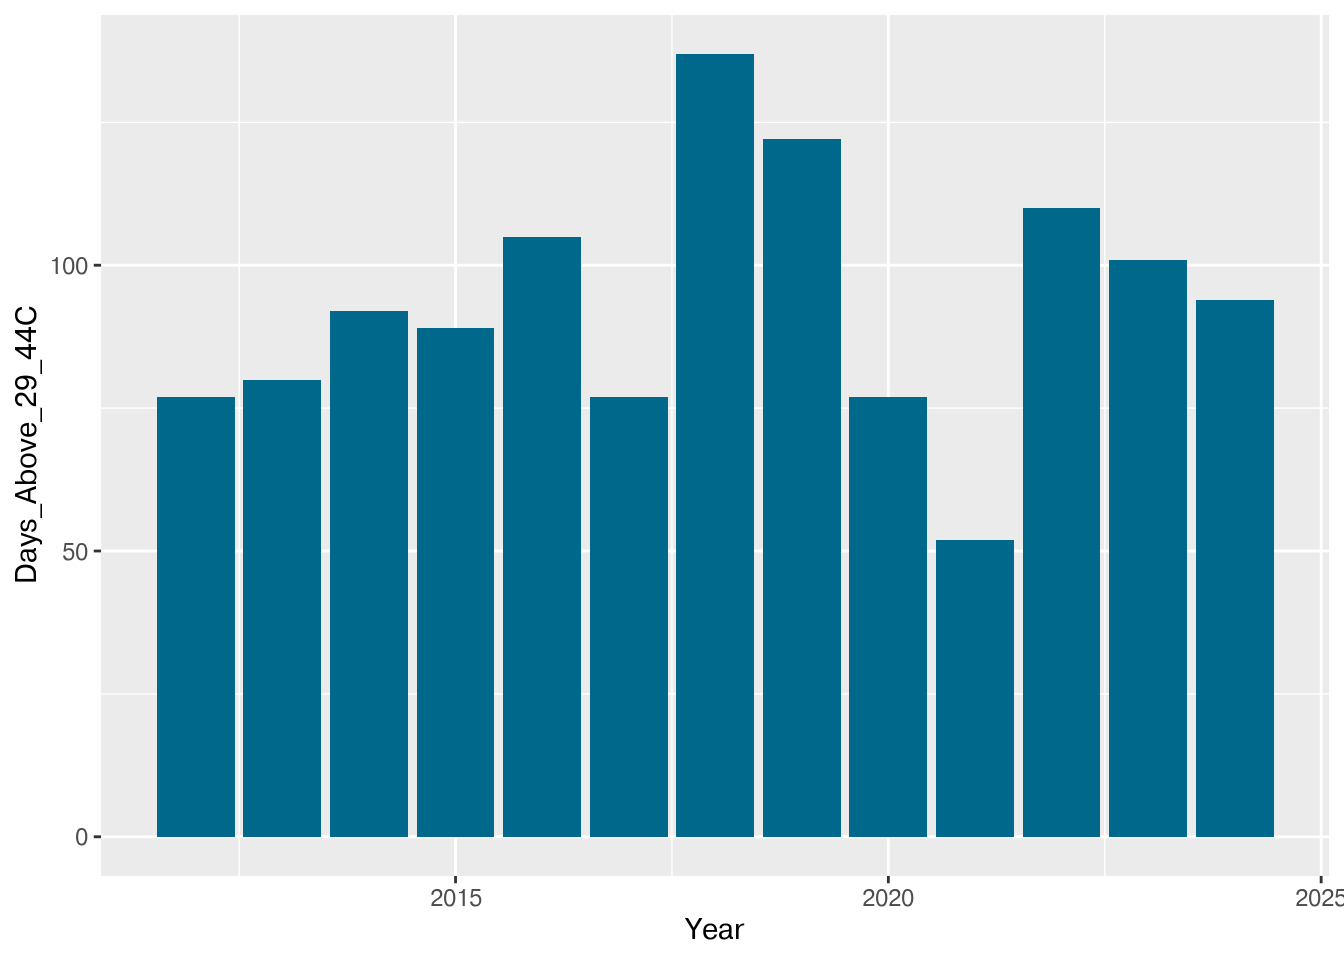
\includegraphics[keepaspectratio]{draft-data-doc_files/figure-pdf/unnamed-chunk-8-1.pdf}}

Max temp per year

\begin{Shaded}
\begin{Highlighting}[]
\NormalTok{water\_model\_max }\OtherTok{\textless{}{-}} \FunctionTok{lm}\NormalTok{(Max\_temp }\SpecialCharTok{\textasciitilde{}}\NormalTok{ Year, }\AttributeTok{data =}\NormalTok{ year\_above\_29)}

\FunctionTok{summary}\NormalTok{(water\_model\_max)  }
\end{Highlighting}
\end{Shaded}

\begin{verbatim}

Call:
lm(formula = Max_temp ~ Year, data = year_above_29)

Residuals:
     Min       1Q   Median       3Q      Max 
-0.99396 -0.33352 -0.08462  0.25495  1.13626 

Coefficients:
              Estimate Std. Error t value Pr(>|t|)   
(Intercept) -309.13187   89.64533  -3.448  0.00544 **
Year           0.16978    0.04442   3.822  0.00283 **
---
Signif. codes:  0 '***' 0.001 '**' 0.01 '*' 0.05 '.' 0.1 ' ' 1

Residual standard error: 0.5993 on 11 degrees of freedom
Multiple R-squared:  0.5704,    Adjusted R-squared:  0.5314 
F-statistic: 14.61 on 1 and 11 DF,  p-value: 0.002834
\end{verbatim}

\begin{Shaded}
\begin{Highlighting}[]
\NormalTok{future\_data\_max }\OtherTok{\textless{}{-}} \FunctionTok{data.frame}\NormalTok{(}\AttributeTok{Year =} \FunctionTok{seq}\NormalTok{(}\FunctionTok{max}\NormalTok{(year\_above\_29}\SpecialCharTok{$}\NormalTok{Year) }\SpecialCharTok{+} \DecValTok{1}\NormalTok{, }\AttributeTok{by =} \DecValTok{1}\NormalTok{, }\AttributeTok{length.out =} \DecValTok{5}\NormalTok{))}

\CommentTok{\# Predict with confidence intervals}
\NormalTok{future\_predictions\_max }\OtherTok{\textless{}{-}} \FunctionTok{predict}\NormalTok{(water\_model\_max, }\AttributeTok{newdata =}\NormalTok{ future\_data\_max, }\AttributeTok{interval =} \StringTok{"prediction"}\NormalTok{)}

\CommentTok{\# Combine predictions with years}
\NormalTok{forecast\_max }\OtherTok{\textless{}{-}} \FunctionTok{cbind}\NormalTok{(future\_data\_max, }\FunctionTok{round}\NormalTok{(}\FunctionTok{as.data.frame}\NormalTok{(future\_predictions\_max), }\DecValTok{1}\NormalTok{))}
\FunctionTok{names}\NormalTok{(forecast\_max) }\OtherTok{\textless{}{-}} \FunctionTok{c}\NormalTok{(}\StringTok{"Year"}\NormalTok{, }\StringTok{"Predicted Highest Temp"}\NormalTok{, }\StringTok{"Lower"}\NormalTok{, }\StringTok{"Upper"}\NormalTok{)}

\FunctionTok{print}\NormalTok{(forecast\_max)}
\end{Highlighting}
\end{Shaded}

\begin{verbatim}
  Year Predicted Highest Temp Lower Upper
1 2025                   34.7  33.1  36.2
2 2026                   34.8  33.3  36.4
3 2027                   35.0  33.4  36.6
4 2028                   35.2  33.5  36.9
5 2029                   35.4  33.6  37.1
\end{verbatim}

Graph of max temp per year

\begin{Shaded}
\begin{Highlighting}[]
\FunctionTok{ggplot}\NormalTok{(year\_above\_29, }\FunctionTok{aes}\NormalTok{(}\AttributeTok{x=}\NormalTok{Year, }\AttributeTok{y=}\NormalTok{Max\_temp)) }\SpecialCharTok{+}
  \FunctionTok{geom\_line}\NormalTok{() }\SpecialCharTok{+}
  \FunctionTok{geom\_point}\NormalTok{(}\AttributeTok{color =} \StringTok{"deepskyblue4"}\NormalTok{) }\SpecialCharTok{+}
  \FunctionTok{labs}\NormalTok{(}\AttributeTok{x =} \StringTok{"Year"}\NormalTok{, }\AttributeTok{y =} \StringTok{"Max. Water Temp °C"}\NormalTok{, }\AttributeTok{title =} \StringTok{"Max. Yearly Water Temp 2012{-}2024"}\NormalTok{) }
\end{Highlighting}
\end{Shaded}

\pandocbounded{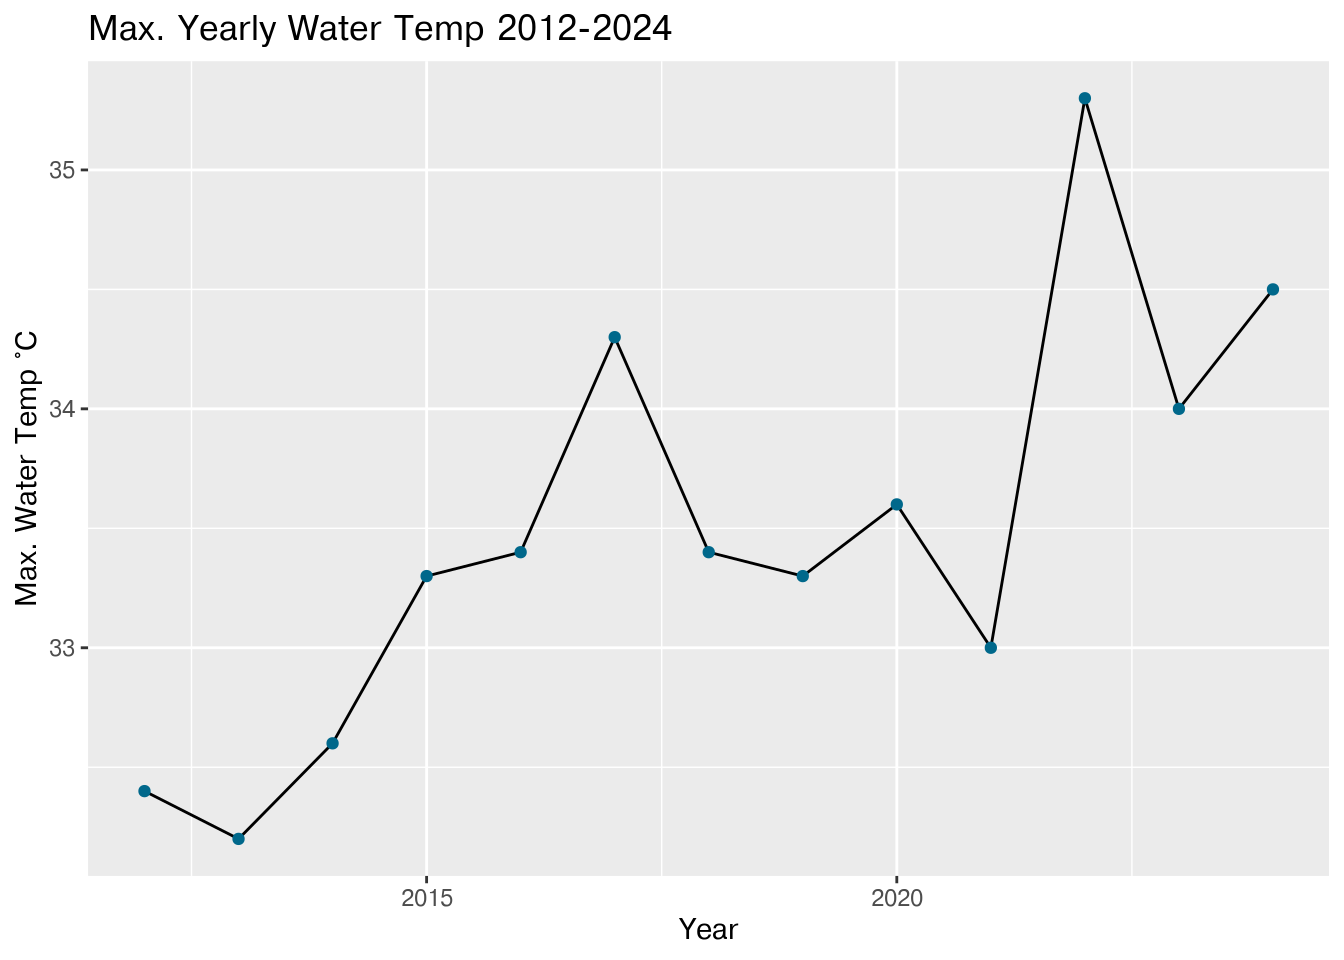
\includegraphics[keepaspectratio]{draft-data-doc_files/figure-pdf/unnamed-chunk-10-1.pdf}}

\#https://www.sciencedirect.com/science/article/pii/S2211467X24000725
This is an article about the dangers of climate change on nuclear
reactors, specifically in the United States. It describes how nuclear
reactors use water to cool themselves down, and if the water temperature
is too high, reactors will have to operate at a lower capacity. It also
shows energy usage in different continents, impacts of lower nuclear
output, and measures to respond for future risks. Portugal-Pereira,
Esteban, and Araújo (2024)

\#https://www.eia.gov/electricity/data/browser/ Has data on electricity
usage, nuclear power output, and state-by-state breakdowns of important
power information. This data can help us determine how heavily a shut
down of the reactor would impact Alabama. {``Electricity Data Browser -
Net Generation for All Sectors''} (2024)

\#https://world-nuclear.org/information-library/current-and-future-generation/cooling-power-plants
Talks about a couple of specific instances where water got too hot and
the plant had to operate on reduced power. The amount of money it cost
consumers is recorded as well as the temperature threshold. There are a
couple of examples and all of them have different limits to how hot the
water can be around their plant. (\textbf{cooling?})

\chapter{Draft: Results}\label{draft-results}

Methods

No data collection was done in our observational study. Everything was
collected from reliable outside sources such as the NOAA and NCEI. This
information was gathered by weather posts in and around Dauphin Island,
measuring ambient water temperature and other important meteorological
observations. While not all days had the same number of water
temperature observations, we were able to use daily averages to make
observations and conclusions about the data.

In our analysis we used the software ``R'' to clean, visualize, and
analyze our information. We created multiple tables to examine daily
average temperatures, yearly maximum temperatures, and prevalence of
days that exceed our thresholds. We also graphed some results to make
them more digestible for a wider audience.

The section discusses an analysis of the risk of shutdown at nuclear
power plants if water used to cool the plant exceeds 85 degrees
Fahrenheit (29.44 degrees Celsius). Using public data, we created an
analysis to find how often the water surrounding Dauphin Island reaches
the 85 degree F threshold and above to help answer our research
question. Below is a table of the mean water temperature each month off
Dauphin Island ({``NCEI Coastal Water Temperature Guide - All Coastal
Regions Table''} 2025).

\begin{longtable}[]{@{}ll@{}}
\toprule\noalign{}
Month & Average WTMP Off Dauphin Island \\
\midrule\noalign{}
\endhead
\bottomrule\noalign{}
\endlastfoot
January & 69.8 \\
February & 69.6 \\
March & 70.6 \\
April & 72.7 \\
May & 78.0 \\
June & 83.4 \\
July & 85.7 \\
August & 86.1 \\
September & 84.3 \\
October & 80.9 \\
November & 76.1 \\
December & 72.3 \\
\end{longtable}

The table below gives the number of days each month in which the average
water temperature exceeded 85 degrees Fahrenheit. Using data from the
NOAA {[}ADD citation when this piece of junk decides to finally load{]},
we found the number of days in each month with an average water
temperature of over 29.44 degrees Celsius (85 degrees Fahrenheit). We
can see that half of June, all of July, much of August, and just over a
week in September recorded an average water temperature above 85. That's
78 days, or 21.37\% of the time. Unsurprisingly, these days are during
the summer, so the power plant would be operating at half capacity
during most of the summer season (is this too Discussiony?)

\begin{longtable}[]{@{}ll@{}}
\toprule\noalign{}
Month & Number of Days With Avg\_WTMP over 29.44 Degrees C \\
\midrule\noalign{}
\endhead
\bottomrule\noalign{}
\endlastfoot
January & 0 \\
February & 0 \\
March & 0 \\
April & 0 \\
May & 0 \\
June & 15 \\
July & 31 \\
August & 24 \\
September & 8 \\
October & 0 \\
November & 0 \\
December & 0 \\
\end{longtable}

To better visualize average water temperature over the course of a year,
we used the same NOAA data as we did in the previous table. Using the
average water temperature from December 2021 to December 2024, we
created a bar graph. The dotted red line represents the 85 degree line.
During the summer months in the middle of the year, there seems to be
many days with an average seawater temperature above the line. We would
highlight these as days of interest.

\pandocbounded{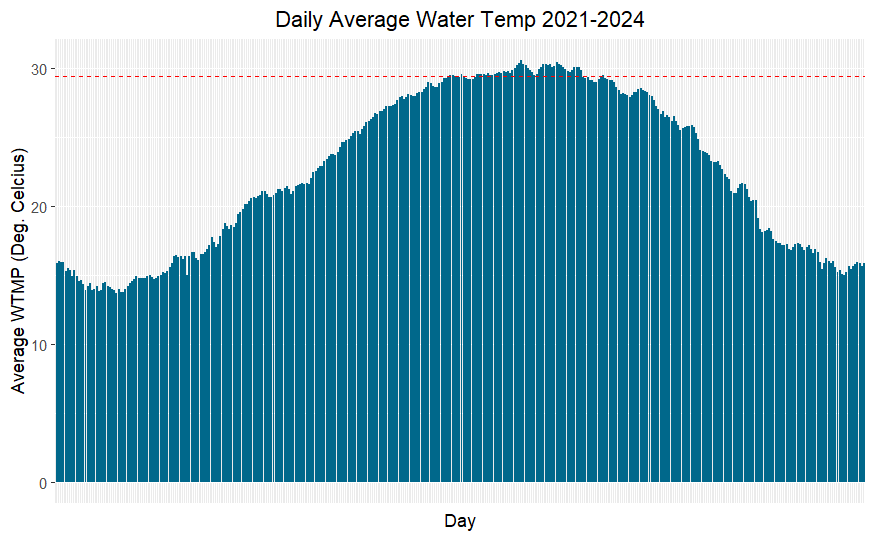
\includegraphics[keepaspectratio]{images/clipboard-3459236136.png}}

Number of Days with an observation of WTMP being greater than 29.44 in
2024

\begin{longtable}[]{@{}ll@{}}
\toprule\noalign{}
Col1 & Col2 \\
\midrule\noalign{}
\endhead
\bottomrule\noalign{}
\endlastfoot
January & 0 \\
February & 0 \\
March & 0 \\
April & 0 \\
May & 7 \\
June & 12 \\
July & 31 \\
August & 31 \\
September & 13 \\
October & 0 \\
November & 0 \\
December & 0 \\
\end{longtable}

Discussion:

To determine the risk of overheating, it's important to find the water
temperature used in cooling the reactor. At the Dauphin Island reactor,
guidelines say the reactor must operate at 50\% capacity when
surrounding waters reach 85 degrees Fahrenheit. The reactor is designed
to use surrounding seawater to cool itself down, but it can't do that
properly if the seawater is too warm. To run our analysis, we must find
the likelihood of the water reaching above the safety threshold.

\chapter{Draft: Intro/Conclusions}\label{draft-introconclusions}

Intro

There are many well-known risks involved with nuclear power generation,
one of those being overheating of the cooling system. In many plants,
water is used to cool the reactor and transfer thermal heat that can be
transformed into electricity. This is crucial in a nuclear power plant,
but if that water is too hot initially, the plant cannot run efficiently
and may damage the surrounding environment. This is what we are trying
to study at the Dauphin Island Nuclear Power Plant on Dauphin Island in
Alabama. What is the risk of the ``cooling water'' getting too hot for
the plant to operate at full capacity?

Multiple studies have found increased water temperature to be
detrimental to the operation of a nuclear power plants across the world.
The World Nuclear Organization details multiple accounts of this
happening in their article on cooling power plants. They say, ``. . .
had to reduce power at its three Browns Ferry units in Alabama to 50\%
in order to keep river water temperatures below 32 degrees Celsius. . .
Rhine and Neckar River temperatures . . . approached the critical 28
degrees Celsius, and nuclear and coal-fired plants were threatened with
closure. In August of 2012 one unit of Millstone power station in
Connecticut was closed because the seawater in Long Island Sound
exceeded 24 degrees Celsius'' (\textbf{cooling?}). This gives us a good
idea of what is to be expected when water temperatures get too high.
However, we want to know about the Dauphin Island plant off the southern
coast of Alabama. There is little to no information about nuclear power
stations in the area that use seawater to cool the reactors, so we hope
to fill in that gap and find the risk of a partial shutdown.

Using data from weather stations in the area, we analyzed the
probability of the Dauphin Island plant having to reduce their
operations due to increased cooling water. Our findings indicated most
summer days reach a temperature above the guideline, forcing our plant
to reduce operations to half . 95\% confidence intervals suggest there
will be a minimum of 30 days worth of shutdowns each of the next five
years, with the potential for up to 170 days. We also found nuclear
power to be a large source of power in Alabama, leading to potential
power outages if the plant were to be forced to function at 50\% output.

Discussion

In order to answer the research question, ``What are the risks
associated with warm water used for reactor cooling at the Dauphin
Island Nuclear Power Plant?'', we must analyze the data we collected
above. The reactor at Dauphin Island is designed to use seawater during
the cooling process. To do so, it collects sea water to pump through the
reactor in order to transfer energy away from the reactor and into the
water, warming it. Warmer water cannot have as much thermal energy
transferred into it as cooler water, and therefore cannot generate as
much power (\textbf{cooling?}). It is also important to note that there
are environmental factors to be considered. A power plant releasing
heated water back into its surroundings can disrupt the ecological
balance, harming or killing the plants and animals in the area. Due to
the potential risks and NRC regulations, once the water temperature
surrounding the plant reaches 85 degrees F, the plant must reduce all
operations to 50\% for the next 24 hours.

In our data collection, we found 94 days in 2024 would have had to
reduce operations at the Power Plant. By cutting power on 25.68\% of the
days, the surrounding areas that rely on the plant for power are now
looking at losing power or having to drastically cut down on their
electricity usage. Using predictive models and confidence intervals, we
can predict the number of ``shutdown days'' over the next five years.
The chart below gives those limits as well as the predicted number of
shutdown days. For example, in 2025, we are 95\% confident the true
number of observed days that water temperature reaches 85° F is between
40.8 and 157.8. It appears the predicted number of days seems to be
increasing by about 1 day per year, but the lower confidence limit is
decreasing while the upper confidence limit is increasing, so we cannot
definitively say if the number of days per year is increasing,
decreasing, or staying the same.

\begin{longtable}[]{@{}
  >{\raggedright\arraybackslash}p{(\linewidth - 6\tabcolsep) * \real{0.0750}}
  >{\raggedright\arraybackslash}p{(\linewidth - 6\tabcolsep) * \real{0.3250}}
  >{\raggedright\arraybackslash}p{(\linewidth - 6\tabcolsep) * \real{0.3000}}
  >{\raggedright\arraybackslash}p{(\linewidth - 6\tabcolsep) * \real{0.3000}}@{}}
\toprule\noalign{}
\begin{minipage}[b]{\linewidth}\raggedright
Year
\end{minipage} & \begin{minipage}[b]{\linewidth}\raggedright
Predicted Number of Days
\end{minipage} & \begin{minipage}[b]{\linewidth}\raggedright
Lower Confidence Limit
\end{minipage} & \begin{minipage}[b]{\linewidth}\raggedright
Upper Confidence Limit
\end{minipage} \\
\midrule\noalign{}
\endhead
\bottomrule\noalign{}
\endlastfoot
2025 & 99.3 & 40.8 & 157.8 \\
2026 & 100.2 & 39.9 & 160.5 \\
2027 & 101.1 & 38.9 & 163.3 \\
2028 & 101.9 & 37.6 & 166.2 \\
2029 & 102.8 & 36.2 & 169.3 \\
\end{longtable}

We also wanted to find the average water temperature for each day to
track potential long-term outages. As is suspected, the summer months
had the most days with water temperatures averaging 85° and higher.
Utilizing the data we collected, we found August to have the highest
average number of days per year that exceeded 85° with 25. July was
close behind at 24 days, while September and June had 2 days a piece. To
make this easier to see, we graphed the average water temperature for
each day in a bar chart. The dashed red line is the 85° threshold, so
any bars that reach above that are days that would be heavily expected
to require a shutdown.

\pandocbounded{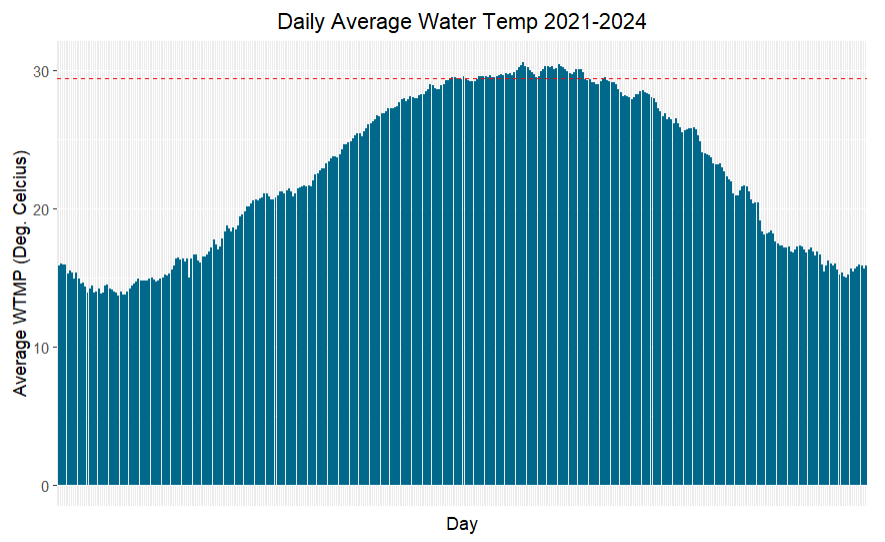
\includegraphics[keepaspectratio]{images/Screenshot 2025-04-16 171204.png}}

According to the U.S. Energy Information Administration, 33\% of the
electricity used in Alabama in 2023 was generated by the two nuclear
power plants in the state (\textbf{u.s.ene?}). Just one of the two
operating at half capacity would have a detrimental effect on consumer
energy use in the state. Residents would have to operate without
certainty of when they'd have power, fearful of outages and relying on
generators during the summer months. Essential businesses such as
hospitals, grocery stores, and pharmacies will take precedent, likely
not losing power completely, but possibly having to cut down on
electrical usage.

Throughout the data collection process, we did our best to reduce any
potential error. Despite using more than a decade of data collected by
the NOAA finding more data that goes back even further would be helpful
in making our results more accurate. We may not get a complete picture
of trends in water temperature, so we may not be able to make
predictions about the future as accurately. In the data we collected,
every day of each year has multiple observations throughout the day, so
we don't have to worry about only observing a maximum or minimum
temperature for that day. It is also important to note that we combined
a few data sets to create our final combined set. All but one year of
data came from the Dauphin Island 1 and 2 meteorological stations, which
are conveniently located less than a mile away from each other. This
difference would likely be negligible and can be ignored. Unfortunately,
the data for 2021 was missing or largely incomplete for every NOAA
station within 20 miles of Dauphin Island, so we had to use data from an
offshore station about 30 ESE of the other Dauphin Island stations. This
data may be different than what was actually observed at Dauphin Island,
so it is important to note that our results may be influenced. We'd much
prefer statistics from Dauphin Island itself in the year 2021, so our
data analysis can be rerun if it is ever uncovered.

It may also be useful to our analysis finding exact data on electricity
output and usage over the last decade or more in Alabama. For the
purposes of this paper, we did not find it to be necessary that we use
exact data. Instead, we cited data from the United States Energy
Information Administration and the World Nuclear Association to make
claims and analyses.

We can connect the data we've collected to previous studies to help
build a better understanding of water temperature in cooling nuclear
reactors. In an article about Climate Resilience, Matthew Bandyk states
the Oyster Creek nuclear power plant was closed, ``rather than spend
\$800 million developing a new water cooing system in order to reduce
the amount of heated water the plant discharged into the local bay. . .
harming the aquatic ecosystem'' (\textbf{fornucl?}). If water
temperatures become too consistently high, it's possible the Dauphin
Island plant may have a future similar to the Oyster Creek plant. The
article doesn't just focus on one power plant though. They found there
to be 17 cases in which a nuclear power plant in the United States had
to reduce operations due to high water temperature in 2019. That number
increased to 25 cases in 2020. Bandyk mentions though, that the trend is
not linear, and can fluctuate based on yearly weather patterns like El
Nino. This data signals shutdowns due to extreme heat are not as rare as
they may initially seem.

This use of water to cool nuclear power plants is not just exclusive to
Dauphin Island, Alabama, or even the United States. Worldwide, this same
system is used. Different countries or regions may have different
guidelines on ideal water temperature, but the idea and consequences are
the same. For example, the World Nuclear Association writes about the
Brown's Ferry Nuclear Power Plant in Northern Alabama, ``In mid 2010,
TVA had to reduce power at its three Brown's Ferry Units in Alabama to
50\% in order to keep river water temperatures below 32 degrees C, at a
cost to some \$50 million to customers'' (\textbf{cooling?}). Worldwide,
almost 10\% of all energy used comes from the 440 nuclear power plants
across the globe (\textbf{nuclear?}). The World Nuclear Association
states that some countries like France, Hungary, or Ukraine, rely on
nuclear energy for more than half of their electricity. In these cases,
the threat of operating at half capacity is more daunting, as it can
effect much of a country's power output.

Despite the research we've done on the topic, there are multiple
opportunities to build on the knowledge we've gained. Using local and
national guidelines, one can research the probability of partial
shutdowns at any nuclear power plant across the world. It may be
particularly helpful to research France's nuclear power plants as they
supply over 70\% of the country's electrical output. A major heat wave
and increase in surrounding water temperatures could lead to ruinous
power outages across the country. Researching the probability of these
outages and the effects they could have is a great first step to
mitigating a country-wide disaster.

Due to increasing concern for the effects of climate change on
environments, we would also recommend further research be done on how
the Dauphin Island power plant may be effected. If water temperature is
increasing on average year-over-year, the power plant could be at risk
for longer periods of working at 50\% capacity, further straining power
supplies in Alabama. Prevention and alleviation tactics would be the
best focuses of future study.

Finally, alternative water sources or water cooling systems could help
ease the stress on nuclear power plants. The use of groundwater is an
intriguing topic, but its slow replenishment could lead to future
resource issues. Rapid cooling of sea water is another interesting idea,
but trade offs must be studied to find the feasibility of this idea.
Upgrading existing cooling features like building a secondary cooling
tower to make the process more efficient should be looked into as well.

\chapter{Draft: Executive Summary}\label{draft-executive-summary}

\chapter{Executive Summary}\label{executive-summary-1}

Intro The Dauphin Island Nuclear Power Plant supplies electricity to
hundreds of thousands of people and businesses across Alabama. Multiple
studies have shown climate change to increase the average air
temperature across the globe, in turn increasing ambient water
temperature. This increasing water temperature in the Gulf of Mexico
around Dauphin Island could harm the plant's ability to run at full
capacity. In fact, any time the surrounding water temperature reaches
85°F (29.44°C), the plant must run at half power to reduce negative
environmental effects.

Methods We used data from weather stations in the Dauphin Island area.
These stations collected atmospheric data as well as water temperature
data, the latter being what we extracted and included in our analyses.
To clean, analyze, and present our data, we used the software package
``R.'' In doing so, we created prjections, confidence intervals, and
graphics that give insights into answering our research question.

Results Our study found there to be a significant chance of a partial
shutdown every year for the next five years. Generated confidence
intervals showed years 2025-2029 are expected to have between 35 and 169
days that reach the 29.44°C threshold, forcing the plant to reduce
operations. {[}Text box of projected days{]} Additionally, the estimated
maximum water temperature reached is expected to increase year over
year. However, the intervals do include temperatures that are lower than
the 2024 maximum. Therefore, we unfortunately cannot make a decision
based on these intervals.

Discussion Based on our results, climate resilience strategies are the
best way to ensure this plant continues operating efficiently. We
recommend doing more research on procedures that can mitigate the risk,
such as sourcing colder water, finding new methods to reuse water, and
increasing turbine efficiency. If no changes are made, many people and
businesses in Alabama could face challenges in being able to use
electricity.




\end{document}
